
%%==================================================
%% demo.tex for BIT Thesis
%%==================================================

% 默认单面打印 oneside 、硕士论文模板 master

\documentclass[oneside, master]{BIT-thesis-grd}

% 模板选项: 硕士论文 master; 博士论文 doctor

%==============更改数学字体设置,Latin Modern Math 默认的的确有点细,看个人需要,下面提供一种方法,需要的可以取消注释=========%

% \usepackage[bold-style=ISO]{unicode-math} %采用unicode-math,可以直接输入Unicode公式,当然传统的输入就行
% \setmathfont{XITS Math}  %目前unicode-math 支持几种数学字体,具体用法可以查看帮助文档,这里采用类似times字体科学数学字体,可以取消注释对比


\begin{document}

%%%%%%%%%%%%%%%%%%%%%%%%%%%%%%
%% 封面
%%%%%%%%%%%%%%%%%%%%%%%%%%%%%%

% 中文封面内容(关注内容而不是表现形式)
\classification{TQ028.1}
\UDC{540}

\title{基于树状区块链的出租车调度算法设计和系统实现}
\vtitle{基于树状区块链的出租车调度算法设计和系统实现}
\author{成佳壮}
\institute{计算机学院}
\advisor{陆慧梅副教授}
\chairman{**教授}
\degree{工学硕士}
\major{电子信息}
\school{北京理工大学}
\defenddate{****年*月}
%\studentnumber{**********}


% 英文封面内容(关注内容而不是表现形式)
\englishtitle{Algorithm Design and System Implementation of Taxi Scheduling Based on Ethereum }
\englishauthor{Jiazhuang Cheng}
\englishadvisor{Prof. Huimei Lu}
\englishchairman{Prof. **}
\englishschool{Beijing Institute of Technology}
\englishinstitute{Computer Science and Technology}
\englishdegree{Master of Engineering }
\englishmajor{Digital Information}
\englishdate{*,****}

% 封面绘制
\maketitle

% 中文信息
\makeInfo

% 英文信息
\makeEnglishInfo

%打印竖排论文题目
\makeVerticalTitle

% 论文原创性声明和使用授权
\makeDeclareOriginal

%%%%%%%%%%%%%%%%%%%%%%%%%%%%%%
%% 前置部分
%%%%%%%%%%%%%%%%%%%%%%%%%%%%%%
\frontmatter

% 摘要
%%==================================================
%% abstract.tex for BIT Master Thesis
%% modified by yang yating
%% version: 0.1
%% last update: Dec 25th, 2016
%%==================================================

\begin{abstract}

车载自组网是在交通环境参与者间构建的开放式网络,可以为用户提供去中心化的数据传输能力。基于车载自组网,可以实现事故预警、辅助驾驶、道路交通信息查询、车间通信和网络接入服务等应用。研发这些应用需要地理信息和交通数据的支持,但信息的垄断会引发不正当牟利和恶性竞争。针对这一问题,本文利用部署在车载自组网上的区块链网络,基于GeoHash矢量地图和基于以太坊的树状区块链平台,开发了一套出租车调度和导航系统以完成出租车的去中心化调度。首先,本文选用GeoHash作为系统中统一的位置信息表示方法,在系统实现上采用浏览器与智能合约相结合的方式,在智能合约端开发了基于GeoHash的路径导航算法和车辆的区域调度算法,解决了车乘分配时的并发冲突问题。在浏览器端实现车辆和乘客的数据采集和乘车业务完整流程的设计。系统充分利用了区块链的性质保证车辆信誉数据的安全性、可溯性和在网络内的同步性。利用GeoHash在地理信息上的计算特性对算法速度进行了优化,并进行了优化后的实验验证工作。最后调节系统的关键参数进行性能优化并进行实验验证,通过真实的地图数据验证了此出租车调度系统的可行性。

\keywords{区块链; 导航; GeoHash }
\end{abstract}

\begin{englishabstract}

VANET is an Ad­hoc networks between participants in trafic and providing decentralized data transmission service. VANET can be uesd in application like accident
warning, drive assist system, trafic information service and Inter­Vehicle Communication. The development of these applications requires the support of geographic information and traffic data, but the monopoly of information will lead to unfair profit-making and vicious competition. In response to this problem, this paper uses the blockchain network deployed on the in-vehicle ad hoc network, based on the GeoHash vector map and the Ethereum platform, to develop a taxi dispatch and navigation system to complete the decentralized dispatch of taxis. First, this thesis use GeoHash for storage and calculation of position. The system in this thesis is made up of browser­side programs and smart contract. On the smart contract side, a GeoHash-based route navigation algorithm and a vehicle regional managing algorithm were developed, which solved the problem of concurrency conflicts in the allocation of vehicles and passengers. The browser side realize vehicle and passenger data collection and design the complete process of ride-hailing business. Blockchain makes this system safe, traceable and synchronized. The speed of the algorithm is optimized by using GeoHash's computing characteristics on geographic information, and the optimized experimental verification work is carried out. Finally, the key parameters of the system are adjusted for performance optimization and experimental verification. The feasibility of the taxi dispatching system is verified by real map data. 

\englishkeywords{blockchain; navigation; GeoHash }

\end{englishabstract}

%% 符号对照表,可选,如不用可注释掉
\input{chapters/denotation}
% 加入目录
\tableofcontents


%加入图、表索引(同时取消图表索引中章之间的垂直间隔)
\let\origaddvspace\addvspace
\renewcommand{\addvspace}[1]{}
\listoffigures
\listoftables
\renewcommand{\addvspace}[1]{\origaddvspace{#1}}



%%%%%%%%%%%%%%%%%%%%%%%%%%%%%%
%% 正主体部分
%%%%%%%%%%%%%%%%%%%%%%%%%%%%%%
\mainmatter

%% 各章正文内容
%%==================================================
%% chapter01.tex for BIT Master Thesis
%%==================================================
\chapter{绪论}
\section{本论文研究的目的和意义}

随着城市交通的逐渐发展,道路网络的复杂度以及车辆保有量日益增长,交通基础设施的建设无法满足需求,给交通流量的管理带来困难。在智能交通系统中,自动化的出租车调度系统可以有效地满足实时的出行需求,为智能交通系统的完善提供技术支持,有效地满足城市交通需求以及交通流量的管理与诱导,能够有效提高用户出行效率。(研究出租车调度系统的目的和意义)在车辆调度领域,目前已有集中式的自动化出租车调度系统\upcite{魏玉光2021自动驾驶出租车调度方法及调度系统}。\par
信息的去中心化管理是一项关键技术。设计去中心化的出租车调度系统可以保障用户信息不被滥用,避免恶性竞争,在提高交通系统中乘客乘车效率的同时,也兼顾了出租车司机收入的公平。例如已有为缓解机场压力而设计的机场出租车调度模型,从机场管理部门的角度统筹部署机场出租车调度管理系统,在一定程度上避免了私营企业通过集中式后台管理的软件产品进行不正当牟利,提高机场和市政部门的工作效率\upcite{邢智璇2021兼顾效率与公平的机场出租车调度管理系统研究}。\par
区块链可以用作去中心化的出租车调度系统的开发平台\upcite{2020Secure},区块链是一种去中心化的共享账本,它可以安全地将简单,连续和经过验证的数据存储在系统软件中。与传统技术相比,区块链具有以下三个优势:\par
一是它不能被伪造,所以更安全。每个人都必须验证自己的身份,然后才能根据专用安全通道访问数据库,添加或获取数据,并保留历史访问数据。\par
第二是具有很强的实用性和可信性。每个节点都将维护一个详细数据账本,并且该数据组仍处于不同对象的控制之下,并且根据共识算法将数据维持在高度一致的水平,增强了系统的健壮性。\par
第三,它具有智能合约和全自动执行功能。智能合约具有完全透明,可靠,强制执行和全自动执行的优势,可以支持构建去中心化的后台系统。\par
利用区块链这一去中心化后台开发自动化的出租车调度系统,可以同时拥有信息保密、系统安全健壮、利益分配公平公正这些优点,有助于解决人们对高可信性的出行软件的需求问题,为推动智慧交通系统的建设添砖加瓦。


\section{国内外研究现状及发展趋势}
关于出租车调度系统的研究,目前已经有工作提出基于区块链的拼车系统模型\upcite{2020Blockchain},考虑了车辆和乘客双方的身份验证,但只是提出了原型理论,没有实现车辆调度流程。另外还有在以太坊平台实现的拼车系统,提出了司机和乘客对互相的信任程度的概念\upcite{2020A},Deng等提出了基于区块链的车载网安全支付方案\upcite{2020Electronic},这些工作侧重于安全性的验证和评估,并没有考虑在实际应用中让分布式节点起到车辆调度和导航服务的作用。本文采用基于GeoHash的矢量地图作为基础数据,然后基于地理信息在树状区块链上实现导航系统,以实现最低路径成本的导航算法。\par

随着通信技术和硬件技术的发展,移动用户剧增,随之交互式信息地图服务需求逐渐增多,矢量数据地图正在兴起。在矢量地图数据中,矢量数据可以在所有放缩水平下以不同的颜色正确显示和区分特征,使地图展现更加丰富\upcite{2015A}。矢量地图数据的编码方式是影响其传输性能从而影响其可用性的关键因素\upcite{2013An}。\par
XML 和 JSON 是 web 应用程序中常用的两种矢量数据编码方法\upcite{2011Improving}。但 XML 使用重量级语法导致其格式复杂且大小较大,不利于地图数据传输。JSON 是一种易于读写的轻量级数据表示格式,GeoJSON 是其中一种轻量级的数据表示方法,用于编码各类地理数据结构,可用于简单表示地理信息\upcite{2015Performance}。\par
传统的矢量地图如 Google Maps\upcite{2013CONTRIBUTED}, 采用二维数据经纬度来表示地理信息。Geohash 是一种新型的地址编码方式,不同的是它使用 Base32 编码成一维的字符串代替二维的经纬度数据,将二维空间查询转换为一维字符串匹配。利用此优势,GeoHash 编码可以实现时间复杂度为 O(1) 快速查询\upcite{2014A}。此外,相比基于 Base4 编码方法的 Bing Maps\upcite{2014Web},GeoHash 编码使用 Base32 编码方法,即同一前缀有 32 个不同子序列,这缩短了一维字符串的长度从而减小了数据存储和传输的成本。根据编码的长短,GeoHash 可以同时表示图块的坐标和索引范围,从而实现两种功能的统一编码。本文所设计系统的地图存储与展现、导航算法的逻辑将统一基于 GeoHash 编码,完全替换传统地图的经纬度数据表示形式,简化了数据传输和算法逻辑,同时方便了区域信息绑定和查询。\par

传统区块链的特点不能满足车联网的特性。一方面,传统区块链吞吐量较小、出块速度慢,需要改善它的结构来提升可扩展性;另一方面,传统区块链与真实世界的联系较弱,而车联网与地理信息有天然联系并且紧密相关,因此传统区块链结构不能很好适应车联网\upcite{2018Cyber}。就目前来说,主流的方案是将区块链的单链结构改良为多链结构。根据多链结构的构成方式的不同,可以将相关工作分为三类:并发多链\upcite{2019Monoxide},层次多链\upcite{2021Multi},智能合约多链\upcite{2020A}。并发多链存在多条子链,每条子链对应一个独立的功能模块,主链只负责维护多条子链的数据一致性;层次多链以层次化的结构组成区块链;智能合约多链通过智能合约来维护多链数据的一致。树状区块链实现了层次化多链,同时将地理位置融合进区块链的数据结构,对区块链的结构进行修改与优化,使其更能适应车载自组网的特性[周畅论文]。本文基于树状区块链设计出租车调度系统,能更快速地查询和利用地理位置信息,提高系统性能。\par

导航系统的核心部分可分为地理基础数据和底层路径规划算法实现,Dijkstra算法是最短路径算法的鼻祖,但其作为最基本的图搜索算法,无法满足地图路径规划对性能的要求\upcite{2012Finding}。目前工业界地图产品主流的路径规划算法有A*算法,CH(Contraction Hierarchies)算法\upcite{2008Contraction}。其中A*算法是应用最广泛的路径规划算法,其使用了启发式算法,比Dijkstra算法速度更快\upcite{2006A};CH算法实现了数据预处理,以减少需要搜索的节点,但其不支持地理信息的实时更新,且不能很好地支持多种道路权重类型。本文基于A*算法设计了可支持GeoHash格式的地理信息的导航算法。

\section{论文的研究内容、贡献和组织结构}
\subsection{论文的研究内容}
(1)为优化区块链对地图数据的处理性能,降低计算量,引入GeoHash矢量地理信息存储,并为前端矢量地图数据渲染工具——leaflet添加支持GeoHash格式的放缩和拖动功能。\par
(2)为解决中心化的打车软件对用户信息进行违规利用、利用信息差进行恶性竞争等问题,本文基于树状区块链设计并实现了去中心化的出租车调度系统。\par
(3)实现出租车调度系统的核心是实现导航算法和车乘匹配算法,然而,树状区块链缺乏基于矢量地理数据的导航算法支持,为解决这个问题,本文在基于以太坊的树状区块链平台设计并实现了基于GeoHash矢量地理数据的导航算法,并在此基础上实现了基于树状区块链的区域调度车乘匹配算法。\par
(4)针对基于GeoHash的距离计算方法,本文通过前缀匹配对算法逻辑进行了优化;同时,本文在对已广泛应用的导航算法进行了修改,使其支持GeoHash的距离计算逻辑,在导航算法中加入可调节的参数增强其适配性;对导航算法和区域调度车乘匹配算法的关键参数进行调优。
\subsection{论文贡献}
(1)完善leaflet工具对GeoHash格式矢量地图展示的支持。\par
(2)提升GeoHash距离计算算法的速度。\par
(3)设计出基于GeoHash的导航算法并进行参数调优。\par
(4)设计出基于树状区块链的区域调度车乘匹配算法并进行参数调优。
\subsection{论文的组织结构}
第一章,介绍导航应用研究现状以及去中心化调度系统对于智能交通和反垄断、反恶性竞争的意义。\par
第二章,对本文涉及的相关工作进行综述,包括基于以太坊的树状区块链、GeoHash地理信息、leaflet渲染工具、出租车调度系统、导航算法。\par
第三章描述系统的框架,包括服务端智能合约的设计结构,和浏览器终端车辆和乘客的设计结构,以及系统的运行流程。\par
第四章详细介绍系统用到的各种技术,包括基于GeoHash的矢量地图存储和展示、基于GeoHash的导航算法设计、基于树状区块链的区域调度车乘匹配算法。\par
第五章,介绍了出租车调度系统的参数调优以及系统在真实数据下的工作状态。
%%==================================================
%% chapter02.tex for BIT Master Thesis
%%==================================================
\chapter{相关工作}
本章对本文研究内容的相关工作进行简要介绍。首先是基于地理位置的区块链,具体涉及传统区块链的性能瓶颈和地理位置区块链的结构特性。第二是GeoHash地理信息,具体介绍GeoHash地理信息便于区域绑定和查询的特点,基于GeoHash的几何原理,以及矢量地图渲染框架leaflet。第三是出租车调度系统的发展现状,并指出其安全性上的不足和解决方法。第四是路径规划算法,介绍路径规划算法的发展种类,对比各种算法的性能和特点,在此基础上找到适合本文出租车调度系统的算法。

\section{矢量地图}
本节回顾和讨论了 Web 终端访问地图数据的应用程序中涉及的矢量地图编码和空间索引方法。然后简单介绍了本文采用的 GeohashTile 系统使用的 Geohash 编码方法和 Leaflet 以及相关工作的比较。\par

\subsection{Geohash 编码}
Geohash编码将纬度和经度分别转换为一组二进制字符串,然后将这两组字符串逐位交叉,生成一组新的二进制字符串。然后将新字符串每五位转成一个十进制数,按顺序转换成base32编码,这样就可以使用用一维数组表示二维数组\upcite{2014A}。\par
% Geohash的划分过程如图1所示。 
GeoHash 是一个能表示任意精度的高效地理编码系统,它使用二分法将指定区域分为网格,每个网格由唯一的编码表示,网络的大小对应的层次不同,编码越长对应的网格越小,层次越低。地理位置区块链使用 GeoHash 地理编码作为基本数据编码方式。建立 GeoHash 与区块以及交易的索引,从而依据 GeoHash 编码直接获取区域交易内容,同时,GeoHash 编码可以通过前缀对区域信息进行绑定,因此通过 GeoHash 编码可以很自然地建立区域层次与子链的联系。

与谷歌地图的编码方式相比,Geohash 将二维空间查询转换为一维字符串匹配。凭借这一优势,Geohash 可以实现时间复杂度为 O(1) \upcite{2014A} 的快速查询。与Bing Maps的编码方式相比,Geohash 采用 Base32 编码方式,即同一个前缀下有 32 个不同的子序列,而 Bing Maps 编码方式是 Base4,即同一个前缀下只有 4 个不同的子序列,所以 Geohash查询更方便。文献\upcite{2014A}还表明,基于 Geohash 的空间索引算法对海量地理数据具有高性能的查询能力。根据编码长度的不同,Geohash可以同时表示图块的索引范围和坐标,实现统一编码。

\subsection{矢量地图数据编码}
矢量数据的编码是影响其传输性能和可复用性的关键因素。XML 和 JSON 是 Web 应用程序中常用的两种矢量数据编码方法\upcite{2011Improving}。XML(可扩展标记语言)\upcite{1997Extensible} 用作 Internet 信息交换的标准。由于 XML 使用的语法不够轻量,不利于 Internet 上的数据传输\upcite{2017Data}。

GeoJSON 是一种用于编码各种地理数据结构的开放标准格式,可用于表示简单的地理特征。GeoJSON 可以比 XML 更方便、更快速地被计算机解析,数据结构更轻量易读\upcite{2015Performance}。GeoJSON 作为一种轻量级的数据编码方法,适用于移动设备之间的数据传输\upcite{2017Tiled}。考虑到编码方式的传输性能、可读性和易分析性,我们选择GeoJSON作为移动设备矢量数据的编码方式。
\subsection{矢量地图空间索引技术}
空间索引技术是提高海量空间数据查询效率的关键技术。空间索引对瓦片金字塔的地理数据进行管理和维护具有重要的作用,其性能直接影响地理信息网络服务的整体性能。其中,网格索引和四叉树索引是瓦片金字塔模型中广泛使用的空间索引方法\upcite{2014A, 2012Spatial, 2009A}。\par
网格索引是按照一定的分辨率等级,将地理信息进行划分并按照矩形网格排列\upcite{Sagan2014Space}。网格索引法要求在查询金字塔中的任何一个瓦片时,只需要查询三个值,即分别代表行、列坐标和缩放级别的X、Y和Z。网格索引是最早的索引方法之一,形式简单。但是,三字段查询也使得它在海量数据的情况下效率低下。\par
四叉树索引以其每个内部节点都有四个子节点命名,是多分辨率在线地图的常用索引方法。该索引方法具有编码简单、易于实现的优点,已被微软必应地图在内的大多数主要网络地图服务提供商采用。\par
谷歌地图的索引方式与网格索引相同。(x, y, z) 三个字段用于表示图块索引值。因此存在海量数据查询效率低的问题。Bing Maps使用(z,quadkeys)两个字段来表示图块索引值,其中 quadkeys 称为四叉树键,通过按位交叉组合将二维块XY坐标组合成一维字符串来优化索引和存储。\par
Geohash 的索引方法是将第 M 层中的一个块划分为第 M+1 层中的 n 个块,所以它也是一种类似四叉树索引方法。与常见的索引结构相比,Geohash 在索引时不需要经过递归计算,因此空间索引只有一层,使得其动态更新更简单\upcite{2014A}。
% 目前,Geohash 已被广泛用于处理具有一维索引的空间数据 [6,22,26,27]。

\subsection{Leaflet矢量地图渲染框架}
Leaflet 是地图的开源 JavaScript 库之一,是 B/S 端 WebGIS 开发项目中广泛使用的开源软件。开发者可以基于库中提供的接口进行开发和扩展,实现地理信息服务的调用和地图数据的基本操作\upcite{2019The}。Leaflet 强大的开源库插件涉及地图应用的方方面面,包括地图服务、数据提供、数据格式、地理编码、地图控制与交互等,也支持自定义控件的实现。这些控件丰富了 Leaflet \upcite{2016Adgt} 的功能。本文的出租车调度系统基于轻量级WebGIS库Leaflet来呈现终端数据,并拓展了其支持GeoHash数据格式的显示功能。

\section{基于以太坊的地理位置区块链}
% 介绍区块链的性能瓶颈,引出地理位置区块链的研究目的、简要介绍原理。
% 地理位置区块链融合了地理信息,分为创世块、分支块(只维护直接下层区域的索引信息)和普通块(记录在对应地理区域内发生的交易)。
区块链是一个共享的不可更改的总账,它用于记录交易、跟踪资产以及建立信任\upcite{王震2019面向大数据应用的区块链解决方案综述}。几乎所有有价值的东西都可以在区块链网络上进行跟踪和交易,从而降低了风险并削减了所有相关成本。区块链是传递交易信息的理想选择,因为它可以提供在不可更改的总账中的即时、共享且完全透明的信息,这类信息同时具备一定的安全性,只能由获得许可的网络成员访问。另外,区块链网络也可以跟踪订单、付款、账户、生产等等,因此可以通过此类技术手段减少不必要的交易纠纷。\par
智能合约是存储在区块链上的程序,可以在满足预定条件的情况下运行,它们通常是自动执行的脚本,以便所有参与者无需任何中介机构的参与就可以立即结果,极大保证安全性。智能合约代码语句十分简单,当预定条件已经得到满足并完成验证时,区块链网络将执行对应动作,比如释放资金,发出凭证等,然后交易完成时更新区块链。由智能合约完成的交易也是无法更改的,只有获得许可的参与者才能看到结果。本文是基于以太坊改进的地理位置区块链平台来设计和部署智能合约,在此基础上进行出租车调度系统的研究。

\subsection{传统区块链的特点和不足}
% 传统区块链的发展,发展到以太坊,以太坊性能上的不足,以及解决以太坊性能的方法。
% 1. 安全性和性能上的不足
% 2. 对地理信息缺乏自有支持
% 3. 要满足车载自组网的灵活和移动特性
% 利用智能合约设计系统
传统区块链技术基于 PoW 共识机制出块无法并发执行,无法满足车载自组网对高并发操作和网络稳定性的需求,传统区块链也不具备移动性,无法与地理位置信息进行绑定,不能有效利用车载网中地理信息的区域化特性。另外,传统区块链的单链结构,要求所有节点必须在同一区块链中,这将会导致节点数目和数据量过大,不满足车载自组网中车辆节点的移动特性,且一旦出现网络分区,就会对整个区块链产生很大影响。目前采用分片技术更改原始单链的链式结构是解决上述问题的主流方法\upcite{2018Blockclique}。当前也有多链结构的相关工作。根据多链结构是否改变底层区块链结构可分为应用多链和结构多链。应用多链,即在应用层面建立不同功能的多个区块链,没有修改底层区块链结构。结构多链,即根据需求对区块链底层结构进行调整的多链结构。
\subsubsection{应用多链}
Shrestha 等\upcite{2019Regional}研究了区域区块链在车载自组网中的应用。由物理边界区域内的节点共享的区块链,区域内部的传播延迟比较小,可以极大减少消息延迟,但此研究并没有设计跨区域和跨链交易的相关内容。\par
Hirtan 等\upcite{2019Blockchain}提出了一种包含专用链和公用链的医疗保健系统。专用链保存患者的真实身份信息;公用链存储患者的健康信息以及临时 ID 数据,实现隐私数据保护和可用数据公开访问。此研究通过特定节点掌握患者临时 ID 和真实身份的关联,来实现两个区块链数据的传递。

\subsubsection{结构多链}
Youngjune 等人\upcite{2019Monoxide}建立多个独立并行的单链共识组。各个共识组地位平等,大部分交易只在组内完成,跨组交易则采用异步方式将中继事务发送到目标区域,而不是整个网络,减轻了网络负载。值得一提的是,为了确保每个区域中的有效采矿能力与整个网络处于同一水平,采用了诸葛弩改进 PoW 的挖矿方式,这也同时保证了分组抵御攻击的能力。但其共识组分区方法没有考虑实际地理位置信息,同时车载自组网中跨区域交易的规模较大,此研究的跨组交易的网络开销较大,不适用于车载自组网。\par
Zamani 等人\upcite{2018RapidChain}提出了基于分片的公共区块链协议,将节点划分为多个较小的称为委员会的节点组,节点组在不相交的交易块上并行操作,并维护不相交的独立账本,也就是分片,分片由每个成员以区块链的形式存储。为了解决节点频繁移入移出对网络造成的影响,将委员会分为活跃和不活跃两个分类,节点创建后,第一次进入委员会需要加入活跃类,再次进入或转移时需要加入不活跃类。但委员会内节点数量固定,缺少灵活性;委员会构建和重构时不涉及地理因素,增加了更新时间,不适用于车载自组网。\par
Byung 等人\upcite{Byung2018Hybrid}将物联网与基于区块链的智能合约相结合,用于结构健康监视 (SHM)。这个区块链物联网网络分为核心和边缘网络。边缘节点充当查询实时响应的集中式服务器,并提供低延迟和带宽使用率,核心网络由具有高存储容量的miner 节点组成,负责生成新块、验证工作证明,并包含自主决策的智能合约,这种划分提高了系统的效率和可伸缩性,但核心网络十分庞大是主要问题。核心网络的庞大影响移动节点的交易效率。\par
Pajooh 等人\upcite{2021Multi}提出了一种多层区块链安全模型来保护物联网网络,同时利用群集的概念来简化多层架构,通过使用模拟退火和遗传算法相结合的混合进化算法来定义物联网 K- 未知簇,选择的群集头负责本地身份验证和授权,增强了网络认证机制的安全性,显示出更适合的平衡网络延迟和吞吐量。但上述两类区块链研究没有考虑到地理因素,跟适用于车载自组网的区块链结构还有一定的距离。\par
Ochôa 等人\upcite{2019A}提出了侧链结构,由 BlockPRI、BlockSEC、BlockTST 三个不同的区块链,使用了三个区块链来确保系统的隐私性,安全性和信任性。BlockPRI 存储每个用户的隐私首选项。BlockSEC 存储用户的数据。最后,BlockTST 管理并验证有关消费者-生产者与消费者-公司之间的能源贸易的信息。为了保证区块链之间的通信,需要通过智能合约维护多链数据一致性。本文吸收了用智能合约自主决策的思想,基于改进的区块链结构和智能合约实现出租车调度系统。
\subsection{地理位置区块链的特性}
车载自组网具备低成本、低时延以及地理位置天然联系的特性,在道路安全等应用提供了重要支持\upcite{2020Application}。区块链作为一种新型的互联网模式,具备去中心化、不可篡改、可追溯等特点,与车联网的联系愈发紧密\upcite{2021Blockchain}。但实际应用上主要包括两个问题,首先,区块链技术通常要求可靠的网络接入,而车载自组网高动态性的接入方式引发的网络不稳定对区块链的应用造成了极大的挑战。其次,车载自组网中的信息通常与地理信息天然绑定,而传统区块链并不支持此特性。因此,研究将地理位置与区块链融合的地理位置区块链[周畅论文]就是为上述灵活性和地理区域问题提供一种可能的解决方案。\par
由于全局同步与共识速度的限制,传统区块链不能很好的适应车载自组网的高动态性,并且不能保证车辆与路侧节点的稳定连接,这将会极大影响到区块链共识机制的可用性。车载自组网与地理信息天然相联,并且车辆通常只需要关注特定区域的信息,而传统区块链记录的交易信息不包含位置,无法根据地理区域查询交易,且传统区块链全局同步的设计会造成网络资源的大量浪费,并且传统区块链无法根据地理信息高效地查询账户和交易相关的数据。地理位置区块链对区块链的结构进行修改与优化,使其更能适应车载自组网特性。地理位置区块链是一种基于位置的区块链[周畅论文],首先,根据 GeoHash 地理编码与地理区域层次关系建立树状结构的区块,同时研究树状结构地理信息相关数据查询速度的优化机制,从而提升区块链在车载自组网中的吞吐量以及与地理信息相关数据的检索速度。因此本文选用地理位置区块链平台来实现分布式的出租车调度系统。\par

\section{出租车调度系统}
% 介绍出租车调度系统的研究现状,
% 1. 指出中心化系统的不足,容易引发信息垄断、信息泄露和恶性竞争。(2篇)
% 2. 非分布式系统,性能问题是瓶颈,未考虑信息加密(1篇)
% 3. 现有的区块链系统。(1篇)
% 4. 采用区块链或者以太坊的系统,但是不够好,比如性能优化不够好,或者功能不够完善(1篇)
随着互联网通信技术的发展,打车软件和其背后的企业以指数级的速度成长,软件平台的即开即用,让乘客主动广播打车需求,方便了居民出行,同时其灵活性和较高的薪酬水平也在吸引全职和兼职司机的不断加入。一项研究\upcite{2016An}表明,对灵活工作时间的向往驱使着司机们和打车平台的企业进行合作。但在鼓励此类企业发展以解决就业和城市管理效率的同时,也应当对其行使的权力进行监管,避免出现敏感信息垄断、滥用、泄露,从而造成难以预计的后果。\par

\upcite{2015The}提到了一种在用车高峰时进行激增定价的策略,目的是提高司机在用车高峰时的工作积极性,满足乘客在高峰期间的多样化乘车需求,所有利益相关者都可以从具有自我调度能力的平台上通过激增定价策略受益。但实际是让打车平台获得了更多攫取利益的空间,使得平台的使命从方便公共交通转向了使自己利益最大化。\par

传统中心化调度系统在存储容量和处理性能方面存在不足,当访问服务器的需求规模扩大后,系统就无法及时处理接收到的需求数据,进而导致响应速度降低和服务质量的下降。随着数据规模的逐渐扩大,单机环境下的处理模式已经不适用于海量数据的存储与计算,分布式存储与计算应运而生\upcite{孙仕亮2017大数据分析的硬件与系统支持综述}。但是事实上,由打车软件提供商设计的分布式系统,其收集和存储到服务器中的用户数据很可能会被泄露给第三方,特别在导航系统中,车辆司机和用户都会提交GPS位置和个人账户信息来获得交通服务和进行导航服务,服务商会出于自己的目的处理用户隐私。\par

文献\upcite{2016Self}的研究将车载网和以太坊结合,实现了透明、自管理的去中心化系统,文章中使用以太坊账户作为车载网中车辆的个人账户,利用智能合约的定制功能,实现个人账户与交通违法行为或税费事物的自动交互,从而实现自管理功能,证明了以太坊平台可以应用于交通领域,但没有实现支持真实交通数据的车辆调度系统。\par

文献\upcite{2018HACIT2}的研究基于Hyperledger Fabric平台,提出了一种使用区块链技术的创新方法,避免了使用第三方软件企业的服务,从而在固定地理区域内实现动态导航路由,同时确也能保用户的匿名性。其不足之处在于,一是作为区块链系统要经常跟第三方库打交道,比如动态路径的生成和改变就依赖在线OSM库,可能导致信息泄露;二是没有充分考虑性能问题,可以利用特殊的地理数据格式来简化算法和存储。采用基于GeoHash的地理信息做存储、导航和调度是不错的改进。

自动驾驶出租车调度模型的关键技术是处理好订单分配和路径规划的问题,然后以此为基础,在时间和空间上对全局需求分布做进一步的优化.

\section{路径规划算法}
% 介绍路径规划算法的发展历史和研究现状,分类简要介绍几种路径规划算法的优缺点,解释为什么有的路径规划算法不适合应用于静态网格道路,指出区块链应用缺乏路径规划算法的支持,以及在区块链中将路径规划算法与GeoHash结合的优点。
% 1. 区分动态和静态路径规划算法
% 2. 解释动态路径规划算法不适用
% 3. 静态算法性能对比
路径规划即通过对道路结构的分析找到最短的路径,最短的概念包括很多维度,比如单纯的从起点到终点的路径长度最短,或者路径的通行时间最短,或者是路径上的路口和交通灯最少等。出租车司机可以根据自己的需求来选择不同类型的最短路径。近几年随着自动驾驶汽车和智能交通系统等概念的炒作,最短路径的求解这一问题的研究热度也随之提升,现有的最短路径规划方法主要分为静态路径规划和动态路径规划两种。\par
静态路径规划算法,即在服务器存储的静态矢量网格地图中寻找从起点到终点的最短路径,可以基于不同的道路权值,计算出该类权值下的最优路径。Dijkstra算法是此类算法的鼻祖\upcite{1959A},Dijkstra算法属于单源最短路径算法,算法规则是从起点开始扩张,向外搜索到达所有节点的最短路径,其时间复杂度是O($ n^{2} $),文献\upcite{2004Taxi}的研究用Dijkstra算法规划了最短路径,设计了基于即时乘车需求和实时路况的路径规划算法。此外,经典的静态路径规划算法还有Floyd算法\upcite{1989A}、A*算法\upcite{1972A},Floyd算法使用的是两个二维数组,它们分别代表图中所有的顶点到所有顶点的最短路径值的总合,以及对应顶点的最小路径的上一跳顶点,此算法考虑到了两点间距离是负值的情况,该算法复杂度是 O($ n^{3} $);A*算法在Dijkstra算法的基础上使用了启发函数,它结合了Dijkstra和启发式算法的优点,以从起点到中间计算点的距离加上该中间点到终点的估计距离之和作为该中间点在优先队列中的优先级,该优先队列在算法执行过程中用来选择中间点的下一跳,A*算法与Dijkstra相比明显降低了时间复杂度。\par
动态路径导航规划方法最早由Cooke and Halsey\upcite{1966The}提出,动态路径规划根据特定类型的道路权值求解起点到重点之间的最短路径,同时实时维护道路信息,对预先规划好的最短路径进行合理的调整,如此维护导航结果直到车辆到达目的地,最终的行车路线即为最优的路径。文献\upcite{孙海鹏2007基于实时交通信息的动态路径规划技术}将实时交通信息动态地记录为该路段的通行时间,以此数据来支持路径规划。\par
文献\upcite{汤永喜2015出租车智能调度终端管理系统的设计与实现}的研究将遗传算法的思想应用到了动态路径规划中,提出了基于动态交通网络模型和遗传算法的最优路径选择算法。但是遗传算法的初始化种群染色体适应度(即连接首尾的路径开销)、“轮盘赌”选择法都增加了不必要的算法负担。且要一直运算到种群中连续N代个体的适应度值基本保持不变,才可选择最优路径,算法开销过大,不适合大规模路段。与Dijkstra算法相比,遗传算法在大型的网格地图中导航容易导致性能瓶颈\upcite{马超2012遗传算法和}。\par
即使是基于实时路况进行路径计算的动态导航,也存在实时交通信息获取的可靠性和准确性问题,以及数据的高效存储和服务器的实时响应等问题,这些问题导致动态路径规划的算法体系不够成熟完善,路径规划的反馈结果不够及时和准确。理论上,遵照这些最短路径算法的结果,就可以得到最优路径的走法。实际上,驾驶员更愿意根据即时有效的路径规划结果来自己判断更有效的路径。本文在地理位置区块链应用中实现了静态矢量地图路网的存储,基于此采用A*算法的思路设计路径规划算法,不同于传统的A*算法,本文在使用 A*算法进行路径规划时支持了GeoHash的数据格式。A*的启发函数基于GeoHash格式进行运算,简化了相比基于经纬度数据的运算量,优化了服务端的存储性能和算法响应速度,更适合分布式和安全性兼顾的出租车调度系统的设计。



%%==================================================
%% chapter03.tex for BIT Master Thesis
%%==================================================
\chapter{基于树状区块链的出租车调度系统框架}
基于树状区块链的出租车调度系统的目标和研发现状简介。

本章介绍了本文所实现系统的框架和流程结构,首先是对系统的架构进行了介绍,包括区块链后台的结构功能,和车辆端和乘客端的终端功能构成;然后对系统的运行流程进行了介绍,包括乘客端的业务运行流程和车辆端的业务运行流程设计。本系统采用本章所描述的结构和流程,结合真实地理数据的矢量地图,模拟了真实地理环境,使系统的运行结果更接近真实环境下的运行情况。

1. 利用树状区块链
2. 利用GeoHash的特性
3. 优化A*路径规划算法
4. 新概念的区域调度
5. 实现去中心化的安全的车辆调度系统
6. 验证基于GeoHash地理数据和区块链研发自组网应用的可行性

\section{基于树状区块链的出租车调度系统架构设计}
介绍基于树状区块链的出租车调度系统的架构,由区块链后台和浏览器客户端构成。
区块链后台是指按一定规律分布在城市交通系统中的路边服务节点,其上运行着自动化执行任务的智能合约。因系统后台是基于树状区块链的,故其可以通过地理信息相关的功能更好地支持整个系统。乘客和车辆的终端分别执行发单和接单的功能,以此和区块链后台一同构成完整的调度系统。乘客和车辆随身运行的终端与其所属区域内的节点服务器进行交互。

\subsection{区块链上智能合约端模块}
介绍区块链后台模块的功能。3段
智能合约运行在树状区块链平台上,根据负责的功能不同分为两种合约,第一种是负责记录地理信息和执行路径规划功能的合约,本章中称其为地图合约;第二种是记录乘客和车辆的身份信息和位置信息的合约,本章中称其为交通合约。将智能合约按功能的类型分开,实现了服务端模块之间的解耦,方便了区块链系统的维护,增加了系统的稳定性和可靠性。

地图合约主要由地图存储模块和路径规划算法模块两个模块构成:
地图存储模块:部署地图合约后,地图存储模块接收JS脚本上传的GeoHash矢量地图,将地图数据与不同前缀长度的GeoHash区域进行绑定,同时,将地图的三叉及多叉路口连接的道路进行存储,以方便路径规划算法在执行过程中对路口所连接道路的查找,客户端可以根据GeoHash区域进行查询,向地图存储合约获取对应的矢量地图并进行展示。

路径规划算法模块:地图合约的路径规划算法模块,是系统进行路径规划的核心部分,其接收一个起点GeoHash参数和一个终点GeoHash参数,通过改进的A*算法进行路径规划运算并返回结果。其中,一对起止点GeoHash既可以由空载车辆当时所处的位置(GeoHash表示)和乘客的上车点位置所组成,也可以由乘客的上车点位置和乘客的目的地位置所组成。路径规划算法返回的结果,是规划出的最短路径上所有路段的起止点构成的一维数组。

除去地图存储和路径规划两个模块外,地图合约还提供了修改算法参数的接口。在以道路长度为权值的路径规划算法中,可以通过接口修改参数从而找到计算性能和准确性最优的参数。除此之外,如果交通场景需求的变化,为导航算法引入了不同类型的权值进行路径规划,此接口也可以方便参数的修改,以方便路径规划算法计算不同权值类型下的最短路径结果,拓展了路径规划模块的健壮性。

交通合约主要由信息记录模块和调度处理模块这两个模块组成:
信息记录模块:在树状区块链上部署交通合约后,车辆和乘客登录终端,然后在智能合约的信息记录模块初始化自己的账户信息和位置信息。在初始化时乘客将自己的乘车状态设置为未乘车,车辆将自己的载客状态设置为未载客。信息记录模块同时也能改变乘客的乘车状态和车辆的载客状态,方便调度处理模块确定可调度的车辆。信息记录模块还会通知相关车辆完成订单后乘客的支付状态,方便车辆司机判断是否可以去接下一单需求。此外,信息记录模块还给司机提供了登出的功能,即车辆司机需要休息或者遇到特殊情况时,可以适时退出调度系统,避免被分配到未来的需求订单。

调度处理模块:交通合约的调度处理模块主要是处理乘客和最近处的车辆匹配的问题。乘客提交打车请求后,调度处理模块会根据乘客的位置,遍历乘客所在区域和相邻区域,寻找到同时满足距离乘客位置最近和空车这两个条件的车辆,然后将其分配给乘客。车辆在接到订单并同意后,调度处理模块会将车辆状态改为已载客。调度处理模块主要完成了寻找区域内最近的车辆和修改车辆和乘客状态这两个功能。


\subsection{浏览器客户端模块}
介绍浏览器客户端模块的功能。3段
乘客在浏览器客户端通过自己的账户信息进行登录,并初始化自己所处的位置(以GeoHash表示位置),然后根据自己的位置通过web3接口从智能合约获取自己位置周边的矢量地图数据,在前端进行展示,乘客可以在渲染的地图中看到自己所处的位置。浏览器端提供了可以使乘客在智能合约记录出发点和终点的模块,然后乘客可以通过manageVehicle功能来向智能合约申请调度车辆,调度成功的车辆位置会在乘客端进行显示。在完成业务后,乘客通过web3接口进行交易确认,同时智能合约会通过监听来确认交易,并通知车辆可以改变自己的状态为空车。

车辆在浏览器客户端通过自己的账户信息进行登录,并初始化自己所在的位置(以GeoHash表示位置),车辆根据自己的位置通过web3接口从智能合约获取周边的矢量地图数据,在前端进行展示,可以看到自己的位置信息。如果司机需要休息或者遇到意外情况,浏览器还提供了退出按钮供车辆退出调度系统,意面接到新的需求订单。在接到乘客订单时,车主可以看到乘客的位置,判断能否顺利接到乘客,如果有困难无法接客可以选择拒绝接受此订单。在确认接受订单后,车辆通过web3接口向智能合约申请到乘客上车点的路径规划;在确认乘客上车后,车辆通过web3接口向智能合约申请到乘客目的地的路径规划。


\section{出租车调度系统流程设计}
出租车调度系统的流程设计,出租车接送客业务的企业研究现状,流程介绍。1段
出租车调度系统的流程
首先乘客通过浏览器客户端发出乘车请求,将自己的起点和终点传到智能合约进行记录。服务器端的智能合约会记录乘客的起始点位置,通过起点的GeoHash获得乘客所在的GeoHash区域,据此进行区域调度来寻找最近的空车,若乘客所在的六位GeoHash区域内没有合适的车辆,则通过GeoHash邻居算法找到乘客起点相邻的8个区域,在这些区域内寻找合适的车辆,然后将最佳匹配的空车的账户id通过web3回调返回给乘客端。

乘客端在收到车辆账户id后,会通知智能合约修改车辆的载客状态和自己的乘车状态。智能合约在接收到车辆账户id后会通过assert检查车辆的载客状态,即检查同一车辆是否在短时间内被分配给了不同的乘客。如果状态检查正常,则智能合约认为车辆和乘客匹配成功,顺利修改乘客的乘车状态和车辆的载客状态;如果状态检查不正确,则智能合约认为这次的车辆调度未成功,会通知乘客端重新进行呼车操作,此过程可隐式进行,方便乘客的操作。通过上述流程可以避免同一车辆被错误分配给多个乘客的错误。

车辆和乘客匹配成功后,相关的车辆会从智能合约监听到自身的状态变化,即智能合约会把乘客的订单通知到对应的车辆。此时司机可以从终端地图上观察到乘客的位置,同时根据自己的条件和意愿判断是否去接送乘客:如果选择不接送乘客,则会将此选择反馈给智能合约,智能合约会通知乘客订单已经被取消,乘客需重新执行呼车流程,同时智能合约也不会再向原车辆提供乘客相关的信息。

如果车辆确认接送乘客,则服务器端的智能合约会根据车辆位置和乘客的上车点执行路径规划,将路径规划的结果进行存储,并将结果通知给车辆端和乘客端,确保双方获取的路径规划结果一致,车乘双方均可在自己的客户端地图观察到路径规划结果。车辆会根据路径规划结果去上车点接到乘客。乘客上车后,车辆确认接到乘客,智能合约会再次执行路径规划算法,通过乘客的上车点和终点得到最优路径,将路径规划结果进行存储,并通知车辆端和乘客端,在双方的地图上显示路径规划结果。车辆会根据最优路径将乘客送到终点。

车辆送乘客到达终点后,乘客执行确认到达终点的操作,表示车辆已经按路径规划结果完成任务。智能合约在接收到乘客的确认到达后,会将乘客的状态从已乘车改为未乘车,将车辆的状态从已载客改为未载客,并更新空车的位置,到此完成了一轮完整的业务流程。车辆在收到智能合约的状态改变通知后,可以根据自己当前的地理位置继续等待下一个订单任务。

\subsection{乘客端业务流程设计}
介绍乘客端浏览器的业务流程。3段
\subsection{出租车端业务流程设计}
介绍出租车端浏览器的业务流程。3段

\section{系统自动化运行框架的设计}
自动化运行框架基于python语法和selenium库实现,通过自动化操作浏览器运行来模拟车辆端和乘客端的行为。
乘客端的自动化python脚本可以通过设置参数来决定打车乘客的数量。自动化脚本控制每个乘客根据自己的账户id登录系统,然后按照各自的起止点需求和发布时间来提出打车请求。在智能合约成功记录乘客的起止点需求后,自动化脚本监听到反馈,会控制乘客端申请车辆调度。匹配到的车辆在确定接单后,会前来上车点接到乘客,并将乘客送到目的地。自动化脚本监听到乘客到达目的地,会执行确认和支付订单的操作,然后退出浏览器客户端,视为乘客完成了一次完整业务。

车辆端的自动化脚本控制每辆车根据自己的账户id登录系统并初始化自己车辆的GeoHash位置,在智能合约进行记录。自动初始化完成后,车辆即可通过监听智能合约的通知来获得乘客订单并选择是否确认接受。车辆可根据即时的乘客需求来执行业务流程。此外,自动化脚本可以控制车辆的工作时长,超出工作时长后,相关车辆将会退出系统,智能合约也不再为其提供乘客订单。


%%==================================================
%% chapter04.tex for BIT Master Thesis
%%==================================================
\chapter{系统的工具和算法原理}

本章对调度系统的区块链服务端和用户端涉及到的算法和工具进行了详细的介绍。服务器端主要涉及地理信息的存储和基于地理信息的算法工作,包括GeoHash静态矢量地图的存储,基于GeoHash静态矢量地图的路径规划算法,筛选最近的空车来与乘客进行匹配的车乘匹配算法。在车辆和乘客的用户端,主要是基于leaflet工具进行GeoHash矢量地图的展示,以及添加相应的功能来优化展示效果。

\section{基于GeoHash的矢量地图展示}

由于终端通信设备的普及和迭代,自组网系统的应用规模不断增大,基于中心化服务器的业务处理速度无法满足网络请求响应的实时性,也限制了自组网车辆之间的通信。而利用区块链的特性实现的分布式后台,既可以保证交易记录的安全性,防止恶意攻击者对地理信息和位置信息、交易信息的篡改,还可以方便成员之间的相互通信,同时其分布式的特性也能够满足对大规模网络请求的及时响应。

本节将介绍GeoHash矢量地图在区块链中的存储逻辑,同时还会介绍在终端页面实现的对GeoHash矢量地图的渲染逻辑,以及为了优化地图展示效果补充的放缩和拖动功能的实现逻辑。

\subsection{基于GeoHash的地图在区块链上的存储}

GeoHash是一种新型的地址编码方式,由Gustavo Niemeyer和G.M. Morton发明[董斌37],其具体算法是二分法结合编码的一种地理位置信息算法[董斌16],被广泛应用到地理位置表示中。最开始,以本初子午线、赤道为界,地球可以分为 4 个部分,设定西经为负,南纬为负,所以地球上的经度范围就是 [-180,180],纬度范围就是 [-90,90]。GeoHash 使用了Peano空间填充曲线\ref{fig:peano},在处理地图数据的过程中,要将经纬度点转换成GeoHash,首先要通过二分的方法把经纬度转化成二进制编码,

% 以 (116.3639092,39.9662639) 为例,将其转化为精度为8位的GeoHash,过程如下表3-1所示(一张表用来示例)。

将经度和纬度分别转换成一组二进制字符串,然后将经度和纬度的二进制字符串以位置交叉的形式进行组码,生成一组新的更长的二进制字符串,新的二进制字符串中偶数位的数字对应原来的经度二进制串,奇数位的数字对应原来的纬度二进制串,然后将新二进制串每五位一组,转为十进制数字,并根据数字找到其在Base32(即数字 0-9 和字母 b-z 不包括 a,i,l,o 的 32 个字符) 数组的映射,以此进行编码[董斌16],最终实现用GeoHash一维数据表示原经纬度二维数据的效果。

\begin{figure}
  \centering
  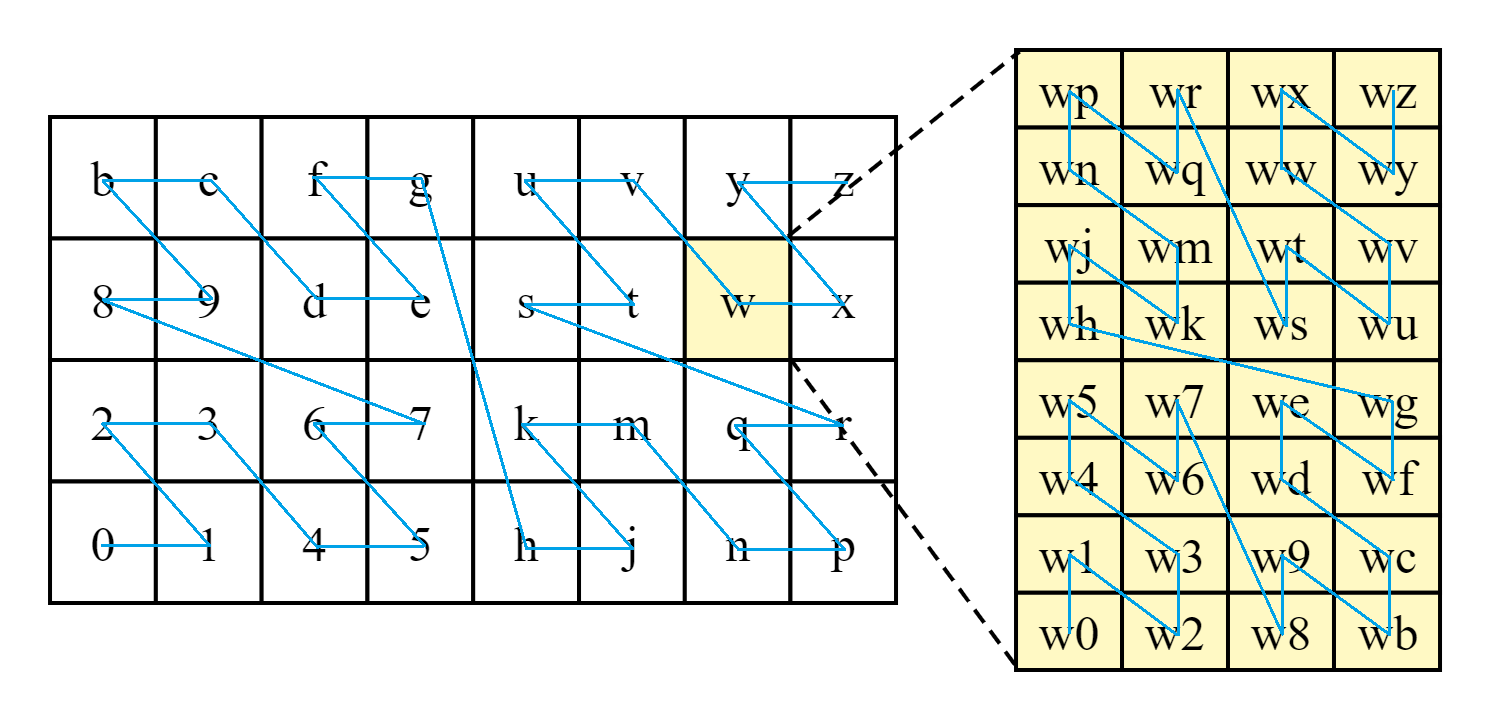
\includegraphics[width=1.0\textwidth]{figures/peano}
  \caption{GeoHash划分和Peano曲线示意图}\label{fig:peano}
\end{figure}


根据Geohash特殊的编码方式,一个GeoHash值对应一个近似矩形的覆盖区域,当位数较短时,它可以表示一块区域的位置,当位数足够长时,它可以表示地球上某个具体点的坐标,重要的一点是,GeoHash位数短的区域一定包含以这个GeoHash为前缀的所有地图数据,如图\ref{fig:fatherAndSon}所示,这一特点对地图数据进行区域绑定提供了极大的便利。GeoHash在编码过程中保留了一定的相对地理位置信息,在大部分情况下,GeoHash编码共同前缀越长的区域相距越近[董斌37],一个6位GeoHash块的覆盖区域大小为1220m*1220m。

\begin{figure}
  \centering
  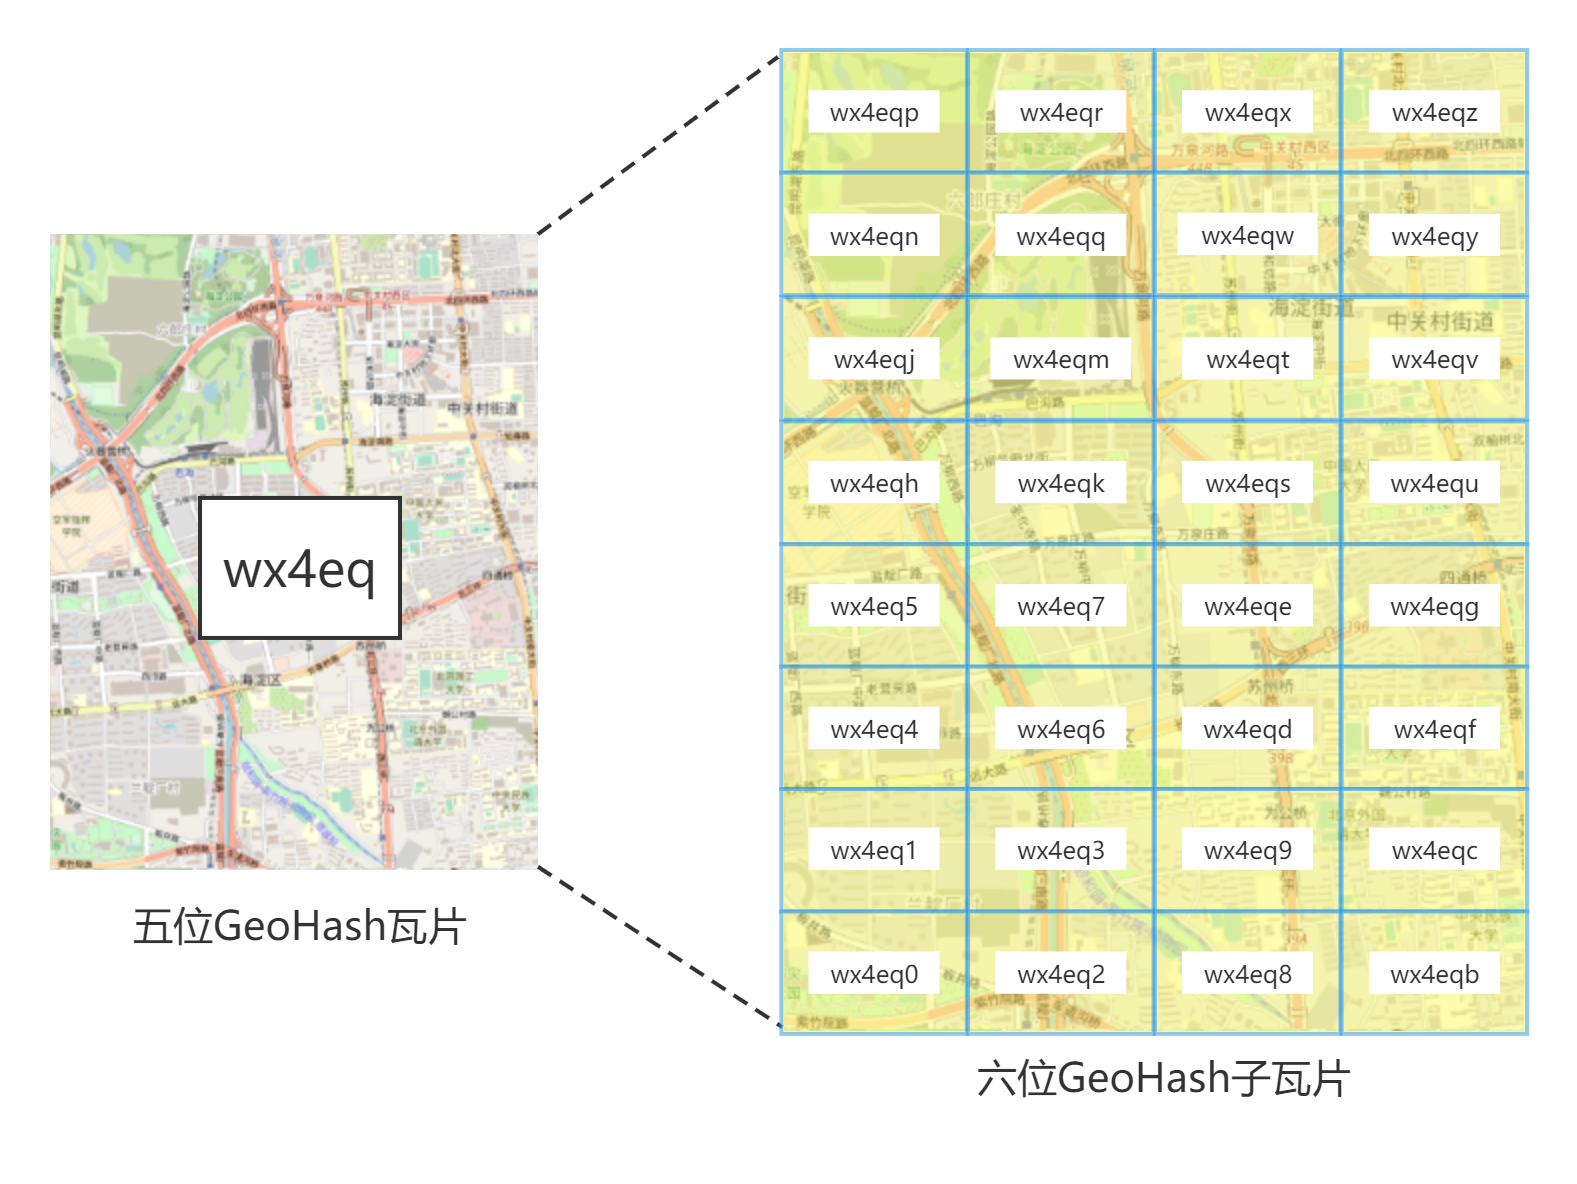
\includegraphics[width=1.0\textwidth]{figures/瓦片与子瓦片}
  \caption{GeoHashTile瓦片与子瓦片的包含关系}\label{fig:fatherAndSon}
\end{figure}


传统的地图数据采用经纬度的方法进行存储,不方便实现位置与区域绑定,并且二维数据存储内容较大,对网络环境和存储设备的要求较高。采用 GeoHash 字符串存储地图信息可以使所有信息平面化,更方便区域信息绑定,并且一维字符串降低了存储数据的规模,同时基于GeoHash地理信息的运算复杂度较低,也更适用于 Solidity 语言。

车辆和乘客的终端在使用时需要从区块链中读取地图信息。为了降低地图数据对终端设备的内存要求,以及降低对网络资源的占用,在区块链存储地图时可将地图进行分块处理,这样终端不用一次读入所有的地图信息。同时,分块后的道路会按照其GeoHash位置的前缀绑定到相应的GeoHash区域内,这样终端在获取地图时能够根据用户的GeoHash位置读入该GeoHash所属的大范围GeoHash区域的地图信息,而不用遍历所有的地图数据,在提高获取效率的同时还会减少网页端的内存消耗,也便于终端地图信息的更新。
% (一张区域绑定示意图)

智能合约中存储的道路信息包括道路ID、道路起点位置、终点位置、道路路径上的点构成的数组(道路为折线段结构)、标识道路间连接信息的 ID(每条道路只在首尾处与其他道路相接)、道路名、道路长度以及单双向行驶标识如表\ref{tab:roadFormat}所示。道路信息属于静态数据,在存储到地图合约的过程中,会对道路末尾连接处所能到达的所有道路的信息记录成一个数组,以方便路径规划算法在运行时对下一条可达道路的启发式查找(记录的算法)。另外,由于开发语言不支持浮点数,因此距离信息需要用GeoHash距离运算的整数结果来表示,此处需要调整运算过程中的参数来找到准确度和运算效率双优的参数。
% (一张参数表)

\begin{table}
  \centering
  \caption{GeoHash道路数据格式}\label{tab:roadFormat}
  \begin{tabular*}{0.9\textwidth}{@{\extracolsep{\fill}}cccc}
  \toprule
    编号    &字段名称 &字段类型 &字段含义 \\
  \midrule
    1    &gid &int &道路id\\
    2    &name &string &道路名称\\
    3    &highway &string &道路类型\\
    4    &cost &int &道路长度(米)\\
    5    &sourceGeoHash &string &道路起点位置\\
    6    &targetGeoHash &string &道路终点位置\\
    7    &source &int &道路起始点的id\\
    8    &target &int &道路终止点的id\\
    9    &oneway &int &道路是否是双向的\\
    10    &coordinates &arraylist &道路路径经过的点\\
  \bottomrule
  \end{tabular*}
\end{table}

\subsection{基于GeoHash的矢量地图的终端数据显示}
[周畅]的GeoHashTile工作设计了基于GeoHash体系的矢量地理数据结构——GeoHashTile,利用了GeoHash对矢量地理数据的高效分区和一维索引,方便对地理数据的查询,并且其支持了对GeoHash地理信息的显示,实现了GeoHash坐标和屏幕上像素坐标的直接转换,并且验证了GeoHashTile在请求数据的速度上比基于经纬度的GeoTile系统有明显优势。其GeoHash转换成屏幕坐标采用的是相对投影的方法。

终端完成显示Geohash矢量地理数据的过程,如图所示,主要包括三个部分:
(1)计算GeohashTile的数量和编码,包括三个步骤:首先获得当前缩放级别下一块GeohashTile的像素大小(每个级别的瓦片像素大小已经通过推理计算设置好[周畅论文]),然后通过屏幕的长宽像素计算客户端中GeohashTile的数量,得到数量后,再通过中心瓦片的GeoHash编码和查找邻居瓦片的算法,计算终端屏幕中所有GeohashTile的编码。
(2)地图数据请求发送到服务端之前,为了减少请求报文的规模,使用GeohashTile请求合并算法来实现要发送的请求的合并。服务器收到请求后会查找请求的所有区域的数据,并整理成基于GeoHash的GeoJSON数据返回给终端。
(3)终端收到地图数据后会进行投影显示,相对位置投影过程包括数据压缩、计算像素距离和计算屏幕坐标三个步骤。实现投影的第一步是计算从这些目标点到中心点的相对像素距离列表。有两种相对距离计算的步骤。第一个是计算从各个GeohashTile中心像素点到屏幕中心像素点的相对像素距离。第二个是计算从目标点的像素点到其所属GeohashTile中心像素点的相对像素距离。将这二者相加即可得到目标点的在屏幕中的像素位置,通过leaflet工具画点的接口进行投影。

% 4.1.1. 计算一块GeohashTile的大小,如步骤1所示?如图5所示。在瓦片地图系统中,瓦片的索引遵循四叉树原则。在每个缩放级别,等式(2)用于计算在x轴和y轴方向上的瓦片数量,其中z是缩放级别。
% 公式(2)
% Geohash编码的每多一个字符就代表将一块区域进行更深层的子分区,一个区域根据编码的奇偶字节交替划分为4×8或8×4子区域。每次分区后对应的x轴和y轴方向上的GeohashTile编码数量的计算公式为公式(3),其中l是Geohash编码的长度。 
% 公式(3)
% GeoHashTile的缩放级别z与GeoHash的字符长度l并不是严格相关的。由于GeoHash每一层的分区都多于GeoTile系统中的四叉树分区,因此,我们结合方程(2)和(3)得到Geohash编码长度l和缩放级别z之间关系的方程(4),在满足公式(4)的基础上,使用最短长度的Geohash编码来做瓦片,以减少存储。对于每个层级z,l的计算结果取最小整数。
% 公式(4)
% 无论谷歌地图、必应地图或其他地理信息显示系统如何,每层的分幅都是固定的像素大小(最常见的分幅像素大小为256×256)。从上面可以看出,Geohash每一层的瓦片大小都是相同的,并且层与层之间的瓦片大小根据划分规则有规律地变化。由于x和y方向的分割大小不一致,Geohash瓦片大多为矩形。为了使GeohashTile在每个级别上近似于256×256的平方像素大小,并便于计算,GeohashTile的像素大小在缩放级别0设置为512×512。结合方程式(4)的计算结果,可通过方程式(5)计算相应缩放级别z下的GeohashTile大小。在等式(5)中,z是缩放级别,l是Geohash编码长度。由于Geohash在x和y方向上的除法规则不一致,因此需要两个不同的方程来完成计算。 
% 公式(5)
% 表3显示了通过等式(5)计算的GeohashTile的像素大小,其中缩放级别为1–18。除了能够计算具有不同编码长度的GeohashTile的像素大小之外,等式(5)还用于稍后计算Geohash坐标点转换屏幕像素坐标。
% 表3
% 4.1.2. 计算客户端中GeohashTile的数量在获得相应缩放级别中GeohashTile的大小后,可以通过组合客户端像素大小来计算屏幕中覆盖的GeohashTile的数量,以便为从服务器获取相应的地图数据做准备(如图5中的步骤2所示)。方程式(6)是计算地砖坐标x轴和Y轴方向上的GeohashTile编码数量的方程式,其中大小为。x、 尺寸。y是客户端屏幕的像素大小。
% 公式(6)
% 为了确保GeohashTile覆盖屏幕,计算结果将被四舍五入。这也是图5所示GeohashTile覆盖范围超出屏幕的原因。

% 4.1.3. 计算客户端中的所有GeohashTile编码以从服务器获得相应的地图数据,我们应该计算屏幕覆盖范围中的所有GeohashTile编码(如图5中的步骤3所示)。

% 4.3 相对位置投影处理所有地图数据都需要从球面数据投影到二维平面数据进行显示。本节描述的Geohash地图数据的相对位置投影过程是使用相对位置计算方法将Geohash编码的地图数据直接投影到屏幕坐标的过程。具体计算步骤如下:

% 4.3.1. 编码长度和缩放级别的关系
% 公式(7)
% 公式(8)
% 这里我们有两个定义来帮助解释。
% 定义1
% 定义2
% 公式(9)
% 4.3.2. 计算相对像素距离
% 算法3

% 4.3.3. 客户端屏幕中心点像素+tile中心点像素偏移+coord相对tile中心点的偏移

\subsection{基于GeoHash的矢量地图实现放缩和拖动功能}

上一节主要讨论了GeoHash矢量地理数据在终端的的投影过程,其核心工作是将GeoHash字符串转投影为屏幕上的像素坐标。本节讲述实现放缩和拖动功能的原理工作,其核心部分的实现逻辑与上一节所述内容相反,实现放缩和拖动功能需要重新设置地图视野的中心点GeoHash,这需要将鼠标在屏幕上的像素点位置转化成相对应地图图层的GeoHash地理位置。(逻辑流程图)

实现GeoHashTile的拖动功能,即通过监听终端操作获得给定的像素值变化,然后对地图进行平移;实现放缩功能,即通过监听终端操作获得缩放等级的变化,然后将地图展示成新的缩放等级。放缩或者拖动结束之后,需要重新获取视野的中心点GeoHash字符串,这个工作是将变化后的地图图层的中心点投影成GeoHash字符串,需要实现将屏幕的像素坐标投影成GeoHash字符串的功能。

首先遍历屏幕内的所有GeoHashTile瓦片,通过(算法1)根据每个瓦片的范围判断操作点所在的瓦片,然后获得该瓦片的中心点GeoHash和中心点像素位置,通过操作点的像素位置和操作点所在的GeoHashTile的像素位置,可以通过(公式1)计算出两点之间的相对像素差,根据相对像素差,结合本缩放层级下的瓦片像素大小,可以通过(公式2)计算出操作点和瓦片中心点在该精度下的GeoHash在东西和南北方向上的地理偏移量(以瓦片中心点GeoHash的精度下所对应的GeoHash格子数表示),根据操作点相对于瓦片中心点的GeoHash地理偏移量,可以通过(算法2)计算出操作点的GeoHash,此GeoHash的精度与瓦片中心点GeoHash相同。(放大缩小示意图)

% 7086_onDragEnd->map.panBy(offset)将地图按给定像素平移

\section{基于GeoHash的几何计算优化}
由于传统计算两个经纬度所表示坐标点距离时需要使用球面距离公式,若在以 GeoHash 为坐标表示的系统中沿用这套算法,则丧失了 GeoHash 带来的计算简便性。利用GeoHash编码的特点进行距离计算,避免了复杂的三角函数和球面计算,并且适用于对小数支持较弱、不提供复杂数学函数计算支持的区块链智能合约编写语言 Solidity。

\subsection{GeoHash几何计算原理}

在将经纬度编码为GeoHash时,首先要将经纬度分别通过二分法编码为对应长度的二进制编码,然后将经度和纬度的二进制编码按照偶数位放经度的二进制编码、奇数位放维度的二进制码的方式进行组码,最后将新获得的组码串进行Base32编码,即可获得GeoHash字符串。

在上述编码的过程中,经纬度二分后对应的两个二进制编码,其对应的十进制值也有特殊的地理意义:即在当前要编码的GeoHash精度下,这一对经纬度对应的GeoHash瓦片,相对于地球原点处所偏移的相同规模的GeoHash瓦片的数量。经度对应的二进制编码的十进制值表示在东西方向上偏移的瓦片数量,纬度对应的二进制编码的十进制值表示在南北方向上偏移的瓦片数量。

根据上述原理,在计算两个GeoHash位置之间的距离时,可以先将两个GeoHash各自解码为在东西和南北方向上表示偏移的数值,再计算这两者在东西和南北方向上偏移的数值之差,即可得到两点之间在东西和南北方向上的相对位置差。由于经纬度划分的原因,在一定的GeoHash精度下,所有瓦片的南北距离都是相同的,但东西距离会根据GeoHash点所在纬度的增加而减小。在10位GeoHash精度下,每个瓦片的东西宽度,可以按纬度的不同大致划分为16个区域。故两个GeoHash点之间的南北距离可以根据南北瓦片的偏差值乘以当前GeoHash精度下瓦片的南北距离(单位:米)获得;而两个GeoHash点之间的东西距离需要根据GeoHash所属的纬度区域找到GeoHash瓦片的东西距离(单位:米),再乘以两者的东西瓦片偏差值获得。

\subsection{GeoHash几何计算方法的优化}
在实际的出租车系统应用环境中,两个终端之间的距离计算所涉及到的地区范围,通常情况下不会超过市辖区以上的规模。故在出租车系统的环境下,两个终端的地理位置GeoHash会有一定位数的前缀是相同的(通常在5位到6位,见表\ref{tab:GeoHashScale})。据此,这两个GeoHash解码后的二进制偏移值的前几位也会相同。事实上二者相同前缀所转化的高位数字是相同的,做减法之后会相互抵消。这些相同前缀转化的的高位数字对二者相对偏移的计算没有影响,这就造成了在GeoHash解码时对计算资源的浪费。

\begin{table}
  \centering
  \caption{GeoHash的长度和距离精度的关系}\label{tab:GeoHashScale}
  \begin{tabular*}{0.9\textwidth}{@{\extracolsep{\fill}}cccc}
  \toprule
    GeoHash长度    &纬度偏差 &经度偏差 &距离偏差(km) \\
  \midrule
    1    &$\pm23$ &$\pm23$ &$\pm2500$\\
    2    &$\pm2.8$ &$\pm5.6$ &$\pm630$\\
    3    &$\pm0.70$ &$\pm0.7$ &$\pm78$\\
    4    &$\pm0.087$ &$\pm0.18$ &$\pm20$\\
    5    &$\pm0.022$ &$\pm0.022$ &$\pm2.4$\\
    6    &$\pm0.0027$ &$\pm0.0055$ &$\pm0.61$\\
    7    &$\pm0.00068$ &$\pm0.00068$ &$\pm0.076$\\
    8    &$\pm0.000085$ &$\pm0.00017$ &$\pm0.019$\\
    9    &$\pm0.000021$ &$\pm0.000021$ &$\pm0.0024$\\
    10    &$\pm0.0000027$ &$\pm0.0000055$ &$\pm0.00060$\\
    11    &$\pm0.00000067$ &$\pm0.00000067$ &$\pm0.000075$\\
  \bottomrule
  \end{tabular*}
\end{table}

在地理视角上,计算两个GeoHash之间的距离,首先是对GeoHash进行解码计算出二者相对地球原点的偏移,如果计算时排除掉两个GeoHash前缀相同的部分,如图\ref{fig:calBetter}所示,此处的参照对象就会从地球原点改为同时包含这两个GeoHash瓦片前缀瓦片(即二者相同前缀部分的GeoHash所表示的瓦片)原点,以距离二者更近的原点作为参照,可以减少计算瓦片偏移数量时的运算规模,从而加快运算速度,使距离计算的算法性能得到提升。

\begin{figure}
  \centering
  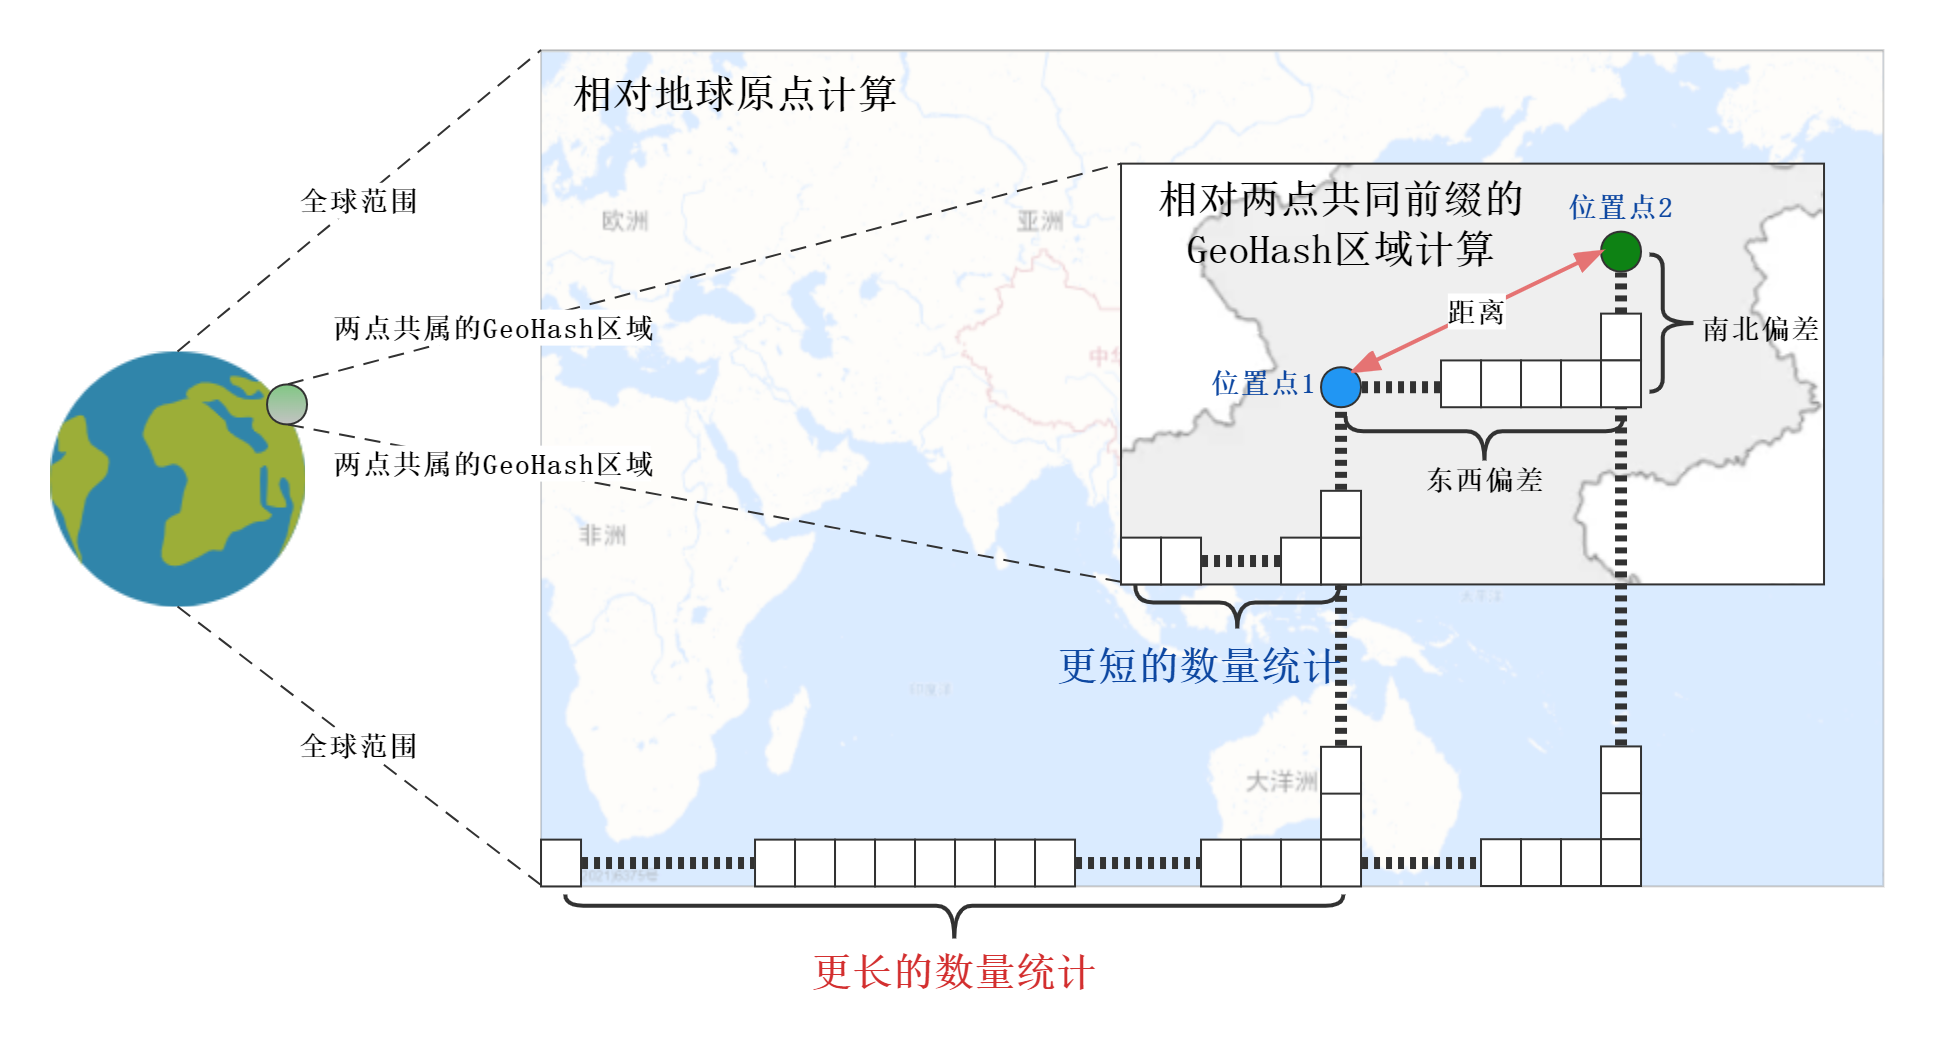
\includegraphics[width=1.0\textwidth]{figures/GeoHash计算优化}
  \caption{GeoHash几何计算优化示意}\label{fig:calBetter}
\end{figure}

本文在进行GeoHash距离计算时,首先检查两个GeoHash的前缀相同的部分,然后取其不同的部分进行距离计算,以优化距离计算的性能,利用了GeoHash字符串的特性,加快系统的响应速度。在智能合约中的算法的逻辑如算法\ref{alg:shortGeoHash}所示,具体的性能优化效果在第五章进行描述。

\begin{algorithm}[t]
  \caption{相同前缀的优化过程算法}
  \label{alg:shortGeoHash}
  \begin{algorithmic}[1]
  \REQUIRE input parameters $geohash1$, $geohash2$
  \ENSURE output $shortGeo1$, $shortGeo2$
  \STATE PRECISION = geohash1.length;
  \FOR{index = 0; index < geohash1.length; index++}
    \IF{geohash1[index] != geohash2[index]}
      \STATE break
    \ENDIF
  \ENDFOR
  \STATE dif = PRECISION - index
  \STATE index2 = 0
  \FOR{j = index; j < PRECISION; j++}
    \STATE shortGeo1[index2] = geo1[j];
    \STATE shortGeo2[index2] = geo2[j];
    \STATE index2++;
  \ENDFOR
  \RETURN shortGeo1, shortGeo2
  \end{algorithmic}
\end{algorithm}

\section{基于GeoHash的路径规划算法}
为了完善去中心化的出租车调度系统,需要在智能合约端实现后台的路径规划算法。路径规划算法的提出和发展由来已久,有适合在未知地图环境下运行的启发式路径规划算法,可以应用在智能机器人和无人车等领域,如机器人的自动寻路、游戏中的AI角色寻路等场景。此外,还有可以在已知地图信息的情况下,利用已有的矢量地图数据规划出最短路径的算法,可以应用在地理信息实时更新的交通系统中,如车载应用的路径规划、公共交通实时路径规划等环境。

本文所描述的系统已有静态矢量地图拓扑信息的支持,故采用静态路网的路径规划算法为车辆提供路径规划的辅助。路径规划算法需要根据智能合约上存储的GeoHash矢量地图数据进行静态导航,参考GeoHash地图存储的格式,在进行地图存储时根据路口的连接关系建立路口之间的拓扑连接关系。本节采用优化后的GeoHash距离计算方法,结合常规静态路网规划算法A*算法,提出了基于GeoHash矢量地图的路径规划算法,为车辆提供路径规划服务。本节实现的路径规划算法可以根据不同的道路权值类型进行路径规划,还可以调节算法参数,在保证路径规划准确性的前提下提高效率。同时,为避免不必要的服务纠纷,会对路径规划的结果进行记录。

\subsection{矢量地图路径路径规划算法的对比选择}

Dijkstra算法是由E.W.Dijkstra于1959年提出,属于贪心算法模式,是非常典型的最短路径算法。此算法可以用于求得移动机器人行进路线中的一个节点到其他所有节点的最短路径。算法的主要特点是:以输入的起始点为中心,算法过程中生成无向图一直向外扩展,直到扩展到最终的目标点为止,通过节点和权值边的连接关系来构成整个路径。Dijkstra算法的缺点是效率低,在无向图扩展的过程中会生成大量的无效路径,占用较多的内存空间。

A*算法(Dijkstra with a Heuristic)是在Dijksra的基础上加入启发式函数实现的,因为加入启发算子的缘故,在拓展无向图的过程中可以根据目标点相对中间点的距离协调选择最好的方向进行搜索。相比Dijkstra算法的效率更高,占用内存空间更少。A*算法的应用范围比较广,可以在电子地图进行路径规划,或者在游戏领域中应用于虚拟角色的行走路径的规划,A*算法的计算结果正确性较高,能够调整算子来适应不同的路径权值类型,拓展了其健壮性和适用范围。

JPS算法在A*算法框架的基础上加入了跳点搜索(Jump Point Search),JPS会根据当前点的方向及当前点周围邻居的特点进行选择,某些特殊的点才能执行加入和删除到可探索点集合的操作。在网格地图中,JPS算法可以用来提高有障碍物时的寻路效率,在遇到障碍物时需要改变搜索方向,这时只把能够以最短路径避过障碍的跳跃点加入可探索点集合中,可以避免考虑很多不必要的路径点,以此来提高算法的搜索效率。但本文的静态地图在储存时已经生成邻居道路的拓扑结构,不需要考虑避开障碍物。JPS算法在已有拓扑结构的地图中徒增算法的复杂度,故不在本文应用。

CH算法在A*算法的基础上加入了预处理的过程,算法在预处理阶段创建“shortcuts”来实现提速,然后在最短路径查询中使用这些“shortcuts”来跳过“不重要的”顶点。“shortcuts”可用于保存两个重要路口之间预先计算的距离,从而算法无需在查询时考虑这些路口之间的完整路径,这样可以使查询路径缩短,查询效率得到提高。但CH算法的预处理使得查询时的道路网络失去了真实的拓扑结构,在每一条道路信息更新后都需要重新对全局进行预处理;此外,道路权值类型的更改也会重新触发整个预处理过程,不能很好地支持实时的交通信息,系统的拓展性和健壮性不足。

\subsection{基于GeoHash的A*路径规划算法的原理}
A*算法是一种直接查询算法,只需要地图的拓扑数据,而不需要做任何预处理。同时 A*算法是一个启发式算法,利用了启发函数,A*算法的启发函数算子可以记成 h(n),代表着算法过程查询到的中间节点到目的地节点的距离估计值。A*算法在选择路径中第n个被检查的节点时,还会参考从起始点到第n个中间节点的实际距离,称为耗散函数,记为 g(n)。A*算法的对中间节点的估计函数(如公式\ref{eqn:calCost})同时参考了耗散函数和启发函数,将二者的和作为评价该节点处于最优路线上的可能性的量度,这样可以首先搜索可能性大的节点。在算法运行的过程中,A*算法根据评估函数f(n)的值,找到距离终点最近的可能性最大的节点,然后展开搜索该节点,而不用每一步规划都需要搜索所有节点,提高了路径规划的效率。

\begin{equation}
  \label{eqn:calCost}
  f(n)=g(n)+h(n)
\end{equation}

A*算法的的核心是设置一个合适的评估函数,评估函数的计算方式对搜索结果有决定性作用。对第n个中间节点来说, g(n) 的值基本是固定的,其反映的是从起点到当前节点的实际道路距离。因此,启发函数 h(n)的选择就显得更重要,它能控制 A*算法计算过程中的行为。如果把 h(n)设置为 0,这时候 f(n)=g(n),A*算法就会退化为 Dijkstra 算法,也能计算出目标路径。启发函数的影响越小,在 A*寻路时需要探索的节点越多,寻路过程就会变慢。启发函数 h(n) 的值如果设置的比 g(n) 大非常多,相当于只有启发函数起作用,A*算法接近 BFS 算法,路径规划的结果不一定是最短路径。
启发函数 h(n) 有以下两个基本的计算距离方法:

(1)欧几里得距离,也叫欧式距离,其计算结果代表两个地理位置之间的直线距离,用M($x_1$,$y_1$)、N($x_2$,$y_2$)两点表示欧式距离的计算公式如下(D表示距离计算结果):

\begin{equation}
  \label{eqn:Euclid}
  D(M, N)=\sqrt{(x_1-x_2)^{2}+(y_1-y_2)^{2}}
\end{equation}

(2)曼哈顿距离,表示在标准坐标系上的绝对坐标轴距之和,曼哈顿距离的计算公式如下:
\begin{equation}
  \label{eqn:manhattan}
  D(M, N)=\mid x_1-x_2 \mid+\mid y_1-y_2 \mid
\end{equation}


本文的实验部分基于GeoHash矢量地图数据,道路属性里的cost字段记录的是道路的实际长度,这个长度即是每条路段的两个端点之间的距离,以米为单位。为了简化启发函数的计算,从而支持智能合约语言的特性,本文采用曼哈顿距离作为度量,结合GeoHash计算距离的函数进行启发函数的计算。为了使启发函数 h(n) 的结果与实际情况更接近,本文调整了GeoHash计算距离函数的参数,使启发函数的结果更接近真实的道路距离,这一步可以让路径规划结果的正确性和算法的效率都得到保障。


\section{基于树状区块链的区域调度车乘匹配算法}

前人工作\upcite{2016A}考虑正常交通对出租车的影响,提出了一种出租车调度系统,该系统使用实时交通状况将空置的出租车与车程最近的等候乘客相匹配。在本文的系统中,在乘客发出乘车请求后,智能合约会根据乘客的位置来为乘客匹配到最近的空车。车辆和用户在初始化自己的信息时,会在智能合约端注册自己的身份和位置信息,智能合约会按照注册的先后顺序对车辆和乘客的信息分别进行记录。在查询空车时,需要按车辆注册的顺序遍历每一辆车,同时查询车辆的载客状态和车辆相距乘客的距离,寻找到距离乘客最近的空载车辆,然后将乘客的请求发送到这辆车的终端,车辆根据乘客的起止点位置来判断是否执行订单。

但是对于大规模应用的系统来书,按注册先后顺序遍历车辆信息的方法显然是低效的,在遍历过程中会查询到较多距离乘客位置较远的车辆,属于无效查询,浪费计算资源,同时也没有利用好分布式系统的特点。树状区块链[周畅论文]将地理信息融合到区块链的分布式系统中,可以根据地理区域快速查询在特定地理区域里的账户信息。故相比传统区块链,融合了地理信息特性的树状区块链能够更好地支持本系统的车辆调度分配工作。

\subsection{树状区块链对区域信息的查询}
\subsubsection{树状区块链结构}
如图\ref{fig:treeBlockchain},树状区块链是基于以太坊的区块链数据结构进行修改的,在其基础上主要新增如下数据结构:
(a) 同层块指针:记录与本区块同层次地理区域对应区块的哈希,与父块哈希一同构成树状区块链。
(b) 位置(\ref{fig:treeBlockchain}蓝色):使用指定长度的 Geohash 编码表示位置,分别在账户状态、交易、收据中新增位置信息,增加账户和交易信息与物理世界的关联。
(c) 区域状态树:以 Geohash 作为索引构建字典树,存储区域内的四种信息:当前区域内的账户(Account)、交易(TXID)、收据(RPID)以及上层区域状态树根节点列表(URRList)记录所有上层区域状态树的根节点哈希,如图\ref{fig:regionState}。
(d) 账户位置树:记录账户发生过的交易所在的区域。可以查询某个账户在指定区域的交易以及历史交易发生的位置, 如图\ref{fig:accountLocation}。

\begin{figure}
  \centering
  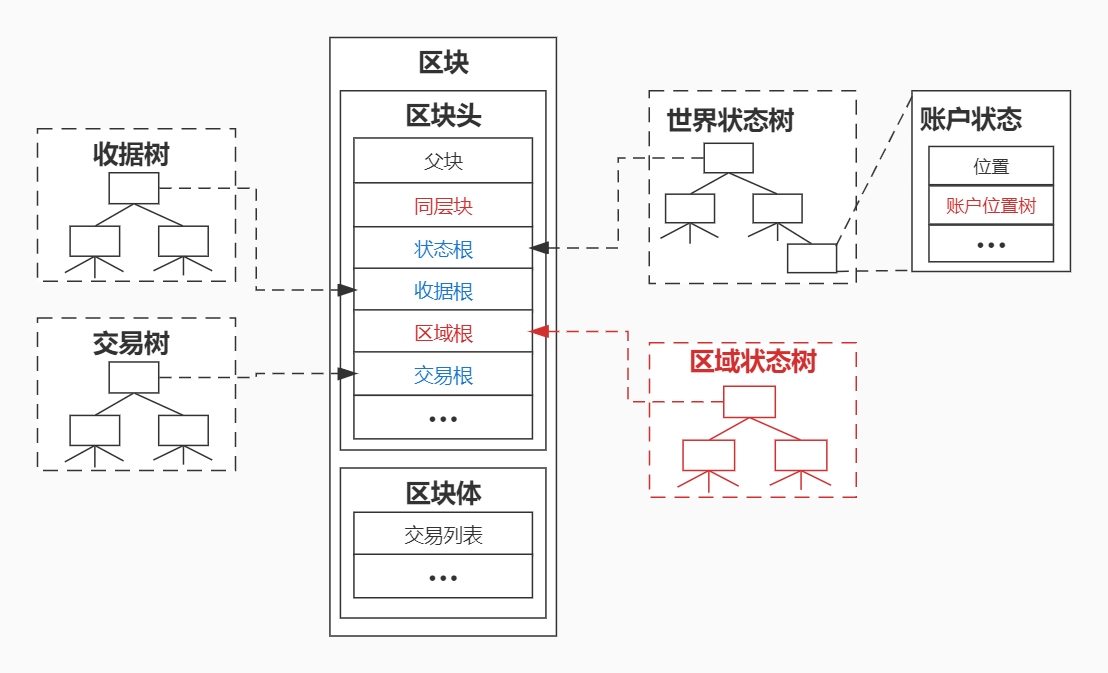
\includegraphics[width=1.0\textwidth]{figures/树状区块链}
  \caption{树状区块链数据结构变化图}\label{fig:treeBlockchain}
\end{figure}

\begin{figure}
  \centering
  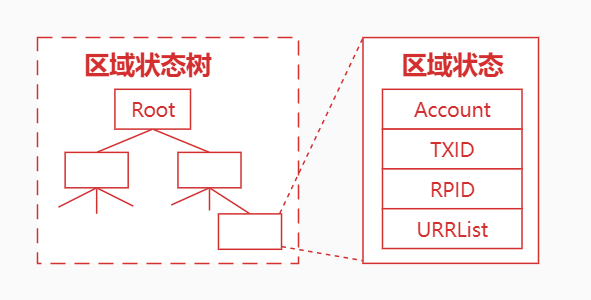
\includegraphics[width=1.0\textwidth]{figures/区域状态树}
  \caption{区域状态树}\label{fig:regionState}
\end{figure}

\begin{figure}
  \centering
  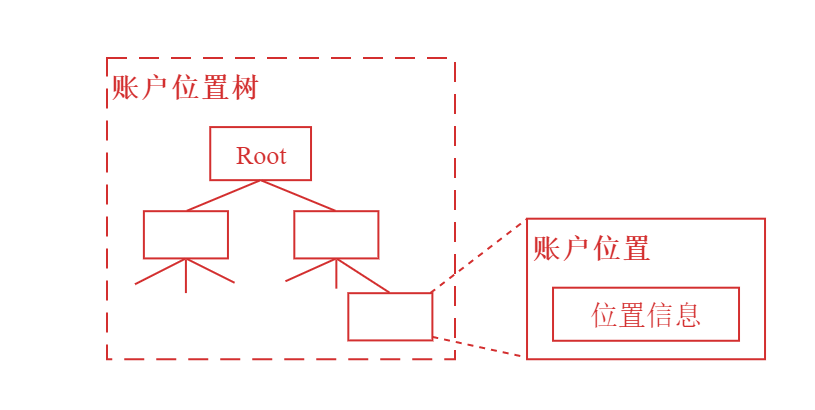
\includegraphics[width=1.0\textwidth]{figures/账户位置树}
  \caption{账户位置树}\label{fig:accountLocation}
\end{figure}

\subsubsection{区块与节点的层次化分类}
为了将区块链划分为树状结构,首先将区块按其特征分为三种:
(a) 创世块:区块链的初始区块。
(b) 分支块:根据 Geohash 编码以层次化结构一一对应创建分支区块作为对应区域内子链的头区块,只维护直接下层区域的索引信息,不记录交易信息。
(c) 普通块:地理区域的最小划分对应分支区块的子区块,记录在对应地理区域内发生的交易。

其次,将网络节点按照其功能分为三种:
(a) 全节点:维护全区块链完整区块数据和全局状态树,部分服务器为全节点。

(b) 区域节点:维护其所在区域内指定层次及以下的所有分支区块与普通区块。每个分支节点负责向上层节点更新汇总当前区域状态并同步所有上层区块链的区域状态树根节点列表。路侧节点与部分服务器为区域节点。
(c) 叶节点:维护所在区域内最下层分支区块以及普通区块。负责局部共识,以及在与区域节点有连接机会时上传缓存信息,并同步所有上层区块链的区域状态树根节点列表。车辆节点为叶节点。
\subsubsection{区块的层次化组织}
在树状区块链设计中,只有普通区块会记录实际发生的交易,分支区块提供子区区块链头区块以及索引功能。每个地理区域都有对应一个分支区块和多个普通区块通过父块哈希指针组成的区块链,同层次不同区域中的分支区块之间通过同层块指针链接起来。分支区块的层次关系代表地理区域的包含关系,即上层分支区块对应的地理区域包含所有以该区块为父块的下层区块对应的地理区域。
树状区块链与传统区块链相比,融合了地理位置,设计了区域状态树和账户位置树等与地理位置相关的数据结构,增加了区块链与真实世界的联系,提升与地理信息相关数据的检索速度。

\subsection{区域调度车乘匹配算法}

利用树状区块链区域状态树查询的特点,可以快速获得区域内的车辆账户信息。当乘客发出乘车请求后,智能合约会根据乘客的位置从树状区块链获得乘客所在区域内的车辆列表,然后根据最近匹配空车的原则从区域的车辆列表中找到最合适的车辆。考虑到区域范围的大小,5位长度的GeoHash所代表的距离范围是2400米左右,而6位GeoHash所代表的距离范围是610米左右,如果考虑的区域范围过大,则涉及到的车辆数量会显著增加,在一定程度上也影响了匹配的速度;如果考虑的范围区域太小,则可能无法找到合适的车辆。

综合上述问题的考虑,结合树状区块链区域查询的优势,本文提出了基于GeoHash邻居查找的区域调度算法,查找的邻居如图\ref{fig:regionManage}所示,系统根据乘客的上车点位置的GeoHash,直接取GeoHash字符串的前缀,可以找到乘客所在位置的GeoHash区域,再根据GeoHash查找邻居的算法找到乘客所在区域以及其周围八个区域共九个区域的GeoHash,从树状区块链的区域状态查询中找到在这些GeoHash范围内的所有车辆信息,然后智能合约会从这些车辆中找到距离最近的空车作为匹配结果。

\begin{figure}
  \centering
  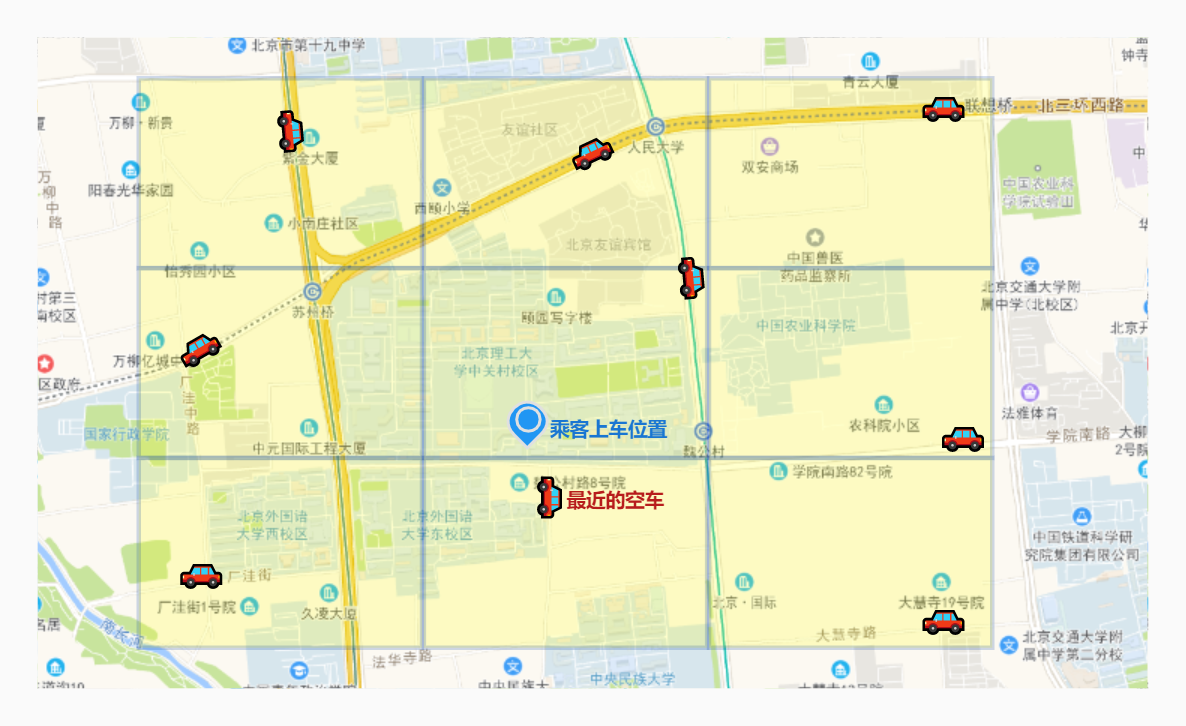
\includegraphics[width=1.0\textwidth]{figures/区域调度}
  \caption{区域调度示意}\label{fig:regionManage}
\end{figure}

在智能合约评估每辆车和乘客的距离时,如果只通过车辆和乘客的GeoHash位置相同的前缀个数来判断距离,由于GeoHash代表的范围随其长度的变化较大,无法对各个车辆的远近做有效的区分,而且\upcite{张海亮2021基于}提出的根据相同GeoHash前缀的长度来判断距离的方法没有考虑到GeoHash的边缘效应(如图\ref{fig:special}所示),无法准确反映车辆和乘客的实际距离。故本系统在评估车辆和乘客距离时采用基于GeoHash的网格距离计算方法,可以通过调节参数在不同规模的GeoHash大小上统计车辆和乘客的距离,可以通过实验选取合适的参数,既保证匹配结果的准确性,也保证计算过程的高效性。

\begin{figure}
  \centering
  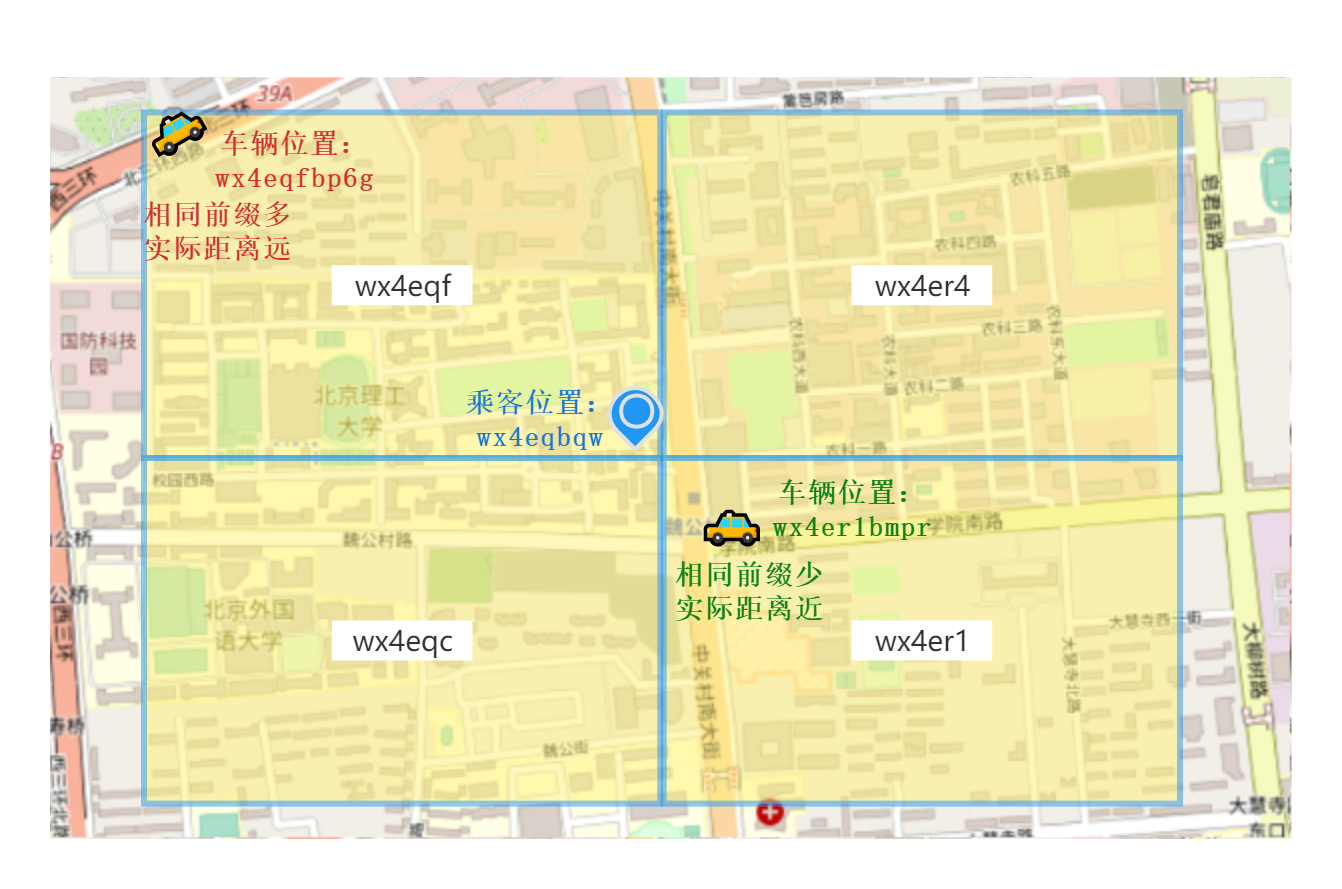
\includegraphics[width=1.0\textwidth]{figures/边缘效应}
  \caption{边缘效应示意图}\label{fig:special}
\end{figure}

本文的区域调度方式可以有效提高车乘匹配的效率,且同时保证了车乘匹配的就近原则,合理地满足了乘客的乘车需求;同时还利用了树状区块链的地理信息特性,通过第五章的实验部分评估了区域调度的正确性和高效性,用实际的应用和实验验证了将区块链与地理信息相结合的技术优势。


%%==================================================
%% chapter05.tex for BIT Master Thesis
%%==================================================
\chapter{实验和系统测试}
上一章对系统所使用的工具和算法原理进行了介绍,为基于GeoHash的矢量地图渲染添加了功能,设计了基于GeoHash的距离计算优化的方法,并在此基础上设计了基于GeoHash的路径规划算法,同时,设计了基于地理位置区块链的区域调度车辆的方法,然后在这些工作的基础上加入真实场景的业务逻辑,实现了完整的出租车调度系统。

本章通过实验对算法的正确性进行了验证,此外还对算法的参数进行对比调节,接着对比了传统区块链环境和地理位置区块链环境所支持的系统的差异,最后分别在模拟网格地图和真实地图上进行了实验,验证本文所实现的调度系统的实用性。

% \section{实验环境说明}


% 张禹:
% 实验环境
% 调节OHMMM算法边界值(一个流程图,三个数据图)
% 近似算法参数优化,设置容量上限为200(一图一表)
% 直接路况精度
%   差错率:带转向延迟的差错率更低,且不带来计算开销(两图)
%   分析了三种车辆异常行为
% 间接补充的路况精度
%   补充路况能够有效提高路况覆盖率(两图)
% 路况结果分析
%   路况统计比轨迹点统计更平滑(一图)
%   统计道路速度(一图)
%   统计路口转向延迟,和道路速度对比关系,证明正确性(一图)
%   展示矢量地图路况(一图)
% 总结

\section{距离计算优化实验}
本节对本文提出的距离计算优化的效果进行实验验证。考虑出租车调度系统的规模,本部分探究了距离在20km内起点和终点距离计算的运算效果。每组实验进行1000次,取结果的平均值。收集优化前后的距离计算算法结果的响应时间和区块链gas消耗,作为对比优化前后性能的参考,结果如图\ref{fig:betterDistance}和\ref{fig:betterGas}。

\begin{figure}[h]
  \centering
  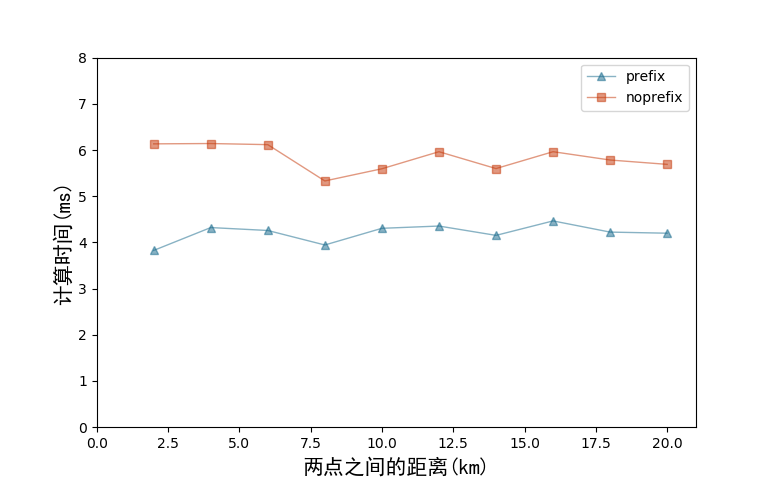
\includegraphics[height=0.3\textheight,width=0.8\textwidth]{figures/距离计算优化时间}
  \caption{距离计算优化前后的时间}\label{fig:betterDistance}
\end{figure}

\begin{figure}[h]
  \centering
  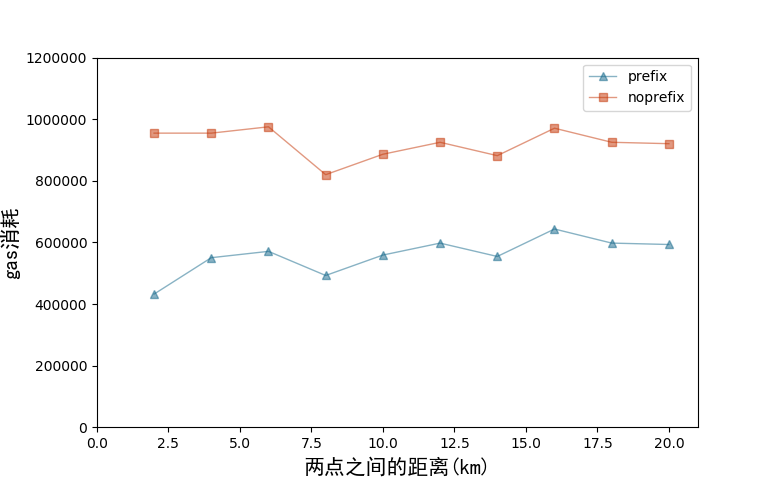
\includegraphics[height=0.3\textheight,width=0.8\textwidth]{figures/距离计算优化gas}
  \caption{距离计算优化前后的gas消耗}\label{fig:betterGas}
\end{figure}

由图分析可知,在20km内不同距离的起止点规模下,前缀优化算法在响应时间上对距离计算的性能提升为28$\%$左右,算法优化后的gas消耗也有明显减少,值得注意的是,算法的计算速度与两点之间距离的远近没有明显的相关性。考虑到GeoHash块的大小,4位GeoHash块的南北长约19.54千米,东西长约28.96千米,因此距离在20km的范围内的两个起止点GeoHash通常前3位及以上的字符是相同的,因此进行计算优化后的优化效果比较明显。但考虑到边界情况,位于GeoHash划分边界的20km范围内的两点GeoHash也有前三位的字符不同的时候。

为了探究边界条件下距离优化算法的表现,本文考虑距离20km内的两点,改变两点相同前缀的位数,收集各个位数下距离计算的响应时间和gas消耗,得到算法优化前后两点GeoHash前缀字符相同的位数与算法运行性能的关系如下图\ref{fig:diffBetterTime}和\ref{fig:diffBetterGas}。

\begin{figure}[h]
  \centering
  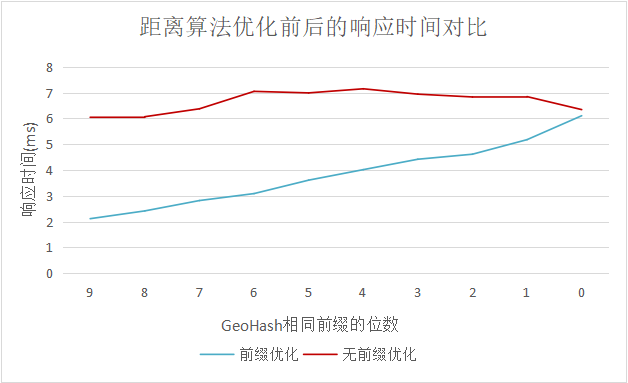
\includegraphics[height=0.3\textheight,width=0.8\textwidth]{figures/不同位数优化时间}
  \caption{不同位数下距离优化的响应时间对比}\label{fig:diffBetterTime}
\end{figure}

\begin{figure}[h]
  \centering
  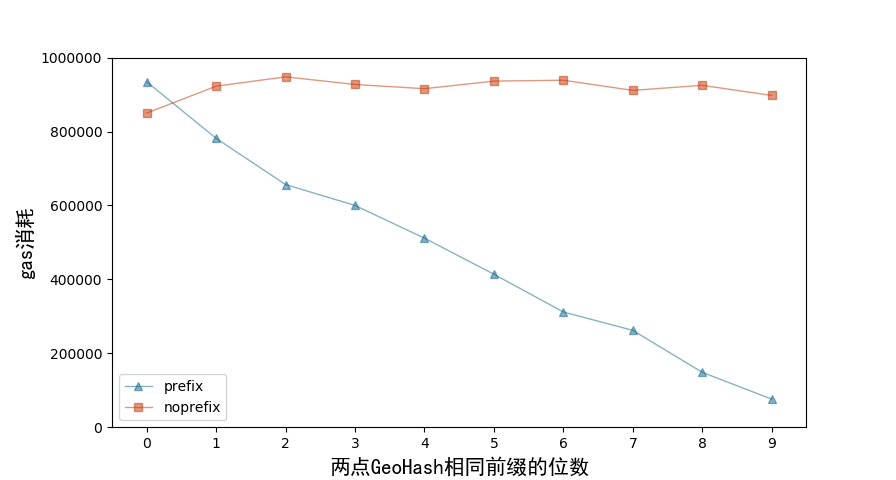
\includegraphics[height=0.3\textheight,width=0.8\textwidth]{figures/不同位数优化gas}
  \caption{不同位数下距离优化的gas消耗对比}\label{fig:diffBetterGas}
\end{figure}

由图中结果可知,在考虑两点在GeoHash划分的边界的特殊情况下,这两个点的GeoHash字符串中前缀相同的位数长短,会影响距离计算的速度。相同的前缀越长,距离计算优化后的计算效率提升越明显。
% 算法正确性实验
%   路径规划算法的路径规划结果正确性展示图(一图,或一模拟图一真实图)

\section{路径规划算法参数实验}
本文用上述优化后的GeoHash距离计算得到的真实地理距离作为astar路径规划算法的启发函数结果。

本节针对不同计算精度下的路径规划算法准确度进行了实验,旨在保证路径规划算法的正确性和结果精度的情况下,提高路径规划算法的计算性能。本实验基于模拟的双行道网格地图,其中每个道路单元的东西主路段长3000m,南北主路段长1100米,路口处的路段长度为40-50米。路径规划算法的启发函数的距离计算精度可以通过调节GeoHash的精度来改变,路径规划算法的计算精度最高到达10位GeoHash。考虑起止点的直线距离在3km到30km内的规模,在此规模内选取不同距离的起止点,通过实验获取路径规划结果的实际路径平均长度和算法平均消耗时间、区块链的gas消耗量,并做对比,找到在保证路径规划正确性的情况下使其计算效率更高的算法参数,实验结果如图\ref{fig:navRoads}、\ref{fig:navTime}、\ref{fig:navGas}所示。

图中nopre代表没有经过距离计算速度优化且计算精度最高(即基于10位GeoHash的格子大小进行计算)的路径规划算法,pre\_10代表距离计算速度优化后且计算精度最高(基于10位GeoHash)的路径规划算法,pre\_9代表基于9位GeoHash格子大小的精度进行计算的路径规划算法,以此类推,pre\_7代表基于7位GeoHash格子大小的精度进行计算的路径规划算法。

\begin{figure}[h]
  \centering
  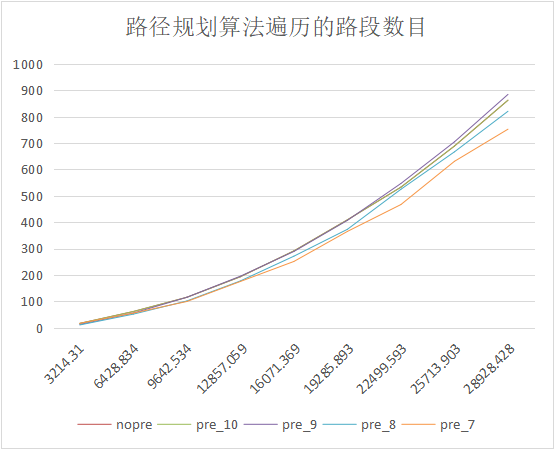
\includegraphics[height=0.3\textheight,width=0.8\textwidth]{figures/路径规划路段数目}
  \caption{路径规划路段数目}\label{fig:navRoads}
\end{figure}

\begin{figure}[h]
  \centering
  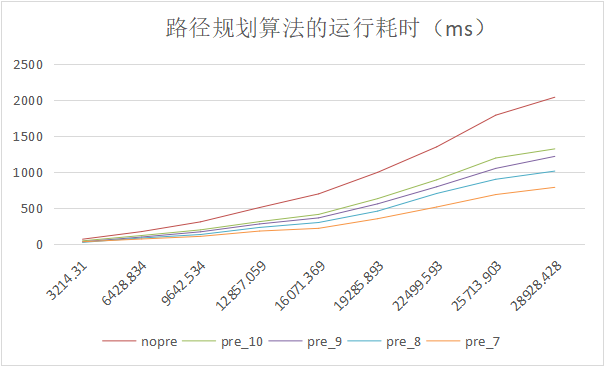
\includegraphics[height=0.3\textheight,width=0.8\textwidth]{figures/路径规划耗时}
  \caption{路径规划耗时}\label{fig:navTime}
\end{figure}

\begin{figure}[h]
  \centering
  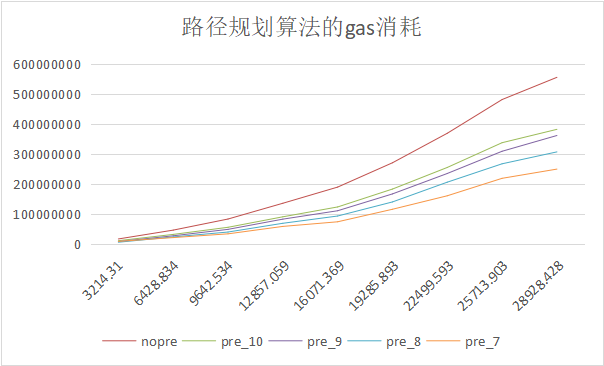
\includegraphics[height=0.3\textheight,width=0.8\textwidth]{figures/路径规划gas}
  \caption{路径规划gas}\label{fig:navGas}
\end{figure}

由实验结果可以看出,有无距离计算速度上的优化,对路径规划算法遍历的路段数目无影响。同时可以发现,距离计算精度的改变,对路径规划算法遍历路段的数目有一定的影响。值得注意的是,计算距离时基于的GeoHash格子规模扩大后,算法遍历的路段数量略有下降(如图\ref{fig:navRoads}),相比pre\_10,pre\_9平均下降了2.21$\%$,pre\_8平均下降了5.87$\%$,pre\_7平均下降了11.29$\%$。这是因为格子规模扩大后,启发函数对各路段相距终点的距离计算结果区分度降低,与终点距离相同的中间路段会增多,而算法在遍历到与终点距离相同的各个中间路段时,不会将其重复加入到算法队列中,如此便降低了算法运行时遍历的路段数目。

区块链执行路径规划算法的gas消耗,随着起止点距离的增加会不断增大,主要是因为起止点之间的路段数目增多,算法遍历的路段数增加,导致后台运算的开销增大。实验收集的数据表明,在没有距离计算优化时,GeoHash的路径规划算法消耗的gas数目明显高于优化后的算法,并且随着起止点之间距离的增加,gas消耗的增长趋势也显著增大。

​在GeoHash距离计算的格子规模不同时,可以观察到,随着GeoHash精度位数的降低,同一对起止点进行路径规划算法的gas消耗会下降,这是因为,距离计算基于格子的规模变大,也就是GeoHash位数减小后,后台的运算量会随之降低,但同时也牺牲了距离计算的精度,用距离计算的精度换取了运算效率的提升。但也不能一味扩大格子的规模,因为7位GeoHash的范围已经达到了50至100米。可以覆盖一个小型路口,如果继续降低GeoHash的位数来增大规模,会明显影响路口处的路径规划精度。
% (实验验证)

实验中统计路径规划算法的运行耗时,以发出起止点请求到收到路径规划结果为止。随着起止点距离的增加,路径规划功能的响应时间会不断增大。在30km的起止点规模下,每一次启发函数的距离计算时间一般不会根据两点之间距离变化受到明显影响。起止点距离增加后,之所以路径规划的响应时间也会增加,主要是因为连接起止点之间的路段的个数变多,导致算法需要遍历的路段个数变多,返回路径规划结果的时间也会随之增加。

根据数据结果可以看出,在距离计算优化前,路径规划算法的响应时间是明显高于距离计算优化后的路径规划响应时间的,距离计算优化后,启发函数计算每条路段与目的地的距离时,运算速度会增加。此外,在GeoHash距离计算的精度不同时,随着GeoHash精度位数的降低,同一对起止点进行路径规划算法的响应时间会降低。

这一方面是因为,距离计算基于的GeoHash精度位数降低,即GeoHash格子规模变大后,进行距离计算的运算量会随之降低,从而缩短了路径规划返回结果的时间。

另一方面,启发函数计算出各路段相距目的地距离的区分度降低,与终点距离相同的中间路段不会重复加入到算法队列中,提高了算法的效率,从而降低了响应时间。

综合考虑运算效率和结果准确度,选取距离计算优化后,GeoHash精度为8时(即prefix\_8)的路径规划算法,可在满足路径规划结果准确度的条件下达到最高的运算效率。从响应时间来看,距离计算优化的使用提升了路径规划算法约35.3$\%$的计算效率,在其基础上,调节计算精度提升了路径规划算法约24.9$\%$的计算效率。

\section{基于地理位置区块链的区域调度实验}

本部分考虑第四章提出的区域查询的边界效应现象,和解决边界效应所提出的邻居区域查询方法。邻居区域查询以乘客位置所在的6位GeoHash区域为中心,根据算法获得其周围的8个邻居区域,地理位置区块链根据这9个区域查询到区域内对应的车辆账户,然后从这些车辆中筛选出距离乘客最近的空车。此查询方法克服单独的6位GeoHash区域查询的边界现象,让车乘匹配的结果更合理。

本部分将对两种方法下的车辆匹配效果进行实验验证。选取4000m × 5000m规模的区域,在区域内随机生成均匀分布的车辆和乘客节点进行匹配,考虑高峰期、平峰期和低谷期三个时刻,高峰期区域内分布200辆车和300个乘客需求,平峰期区域内分布200辆车和200个乘客需求,低谷期区域内分布100辆车和100个乘客需求。收集的数据为乘客相距匹配到的车辆的距离。对比6位直接区域查询到的车辆和6位邻居区域查询到的车辆距离乘客上车位置的平均距离,分析哪种区域查询方法更适合车辆调度。
% 对比6位区域调度和6位邻居区域调度的车乘匹配效果,响应时间对比、车辆到乘客的距离对比(两图)

\begin{figure}[h]
  \centering
  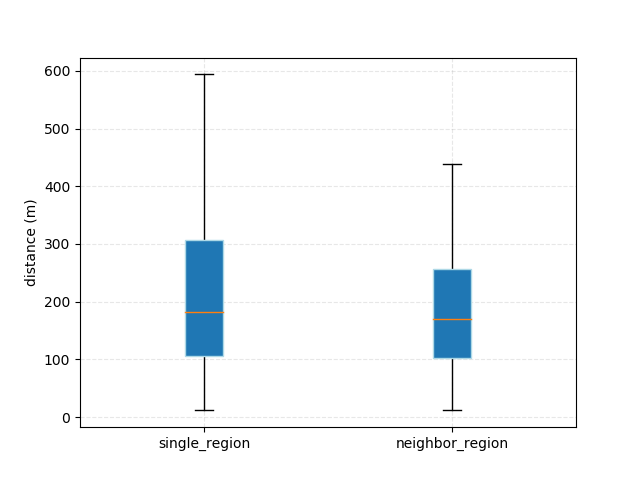
\includegraphics[height=0.3\textheight,width=0.7\textwidth]{figures/高峰车乘匹配}
  \caption{高峰期单独区域调度和邻居区域调度车乘距离对比}\label{fig:highRegionDistance}
\end{figure}

\begin{figure}[h]
  \centering
  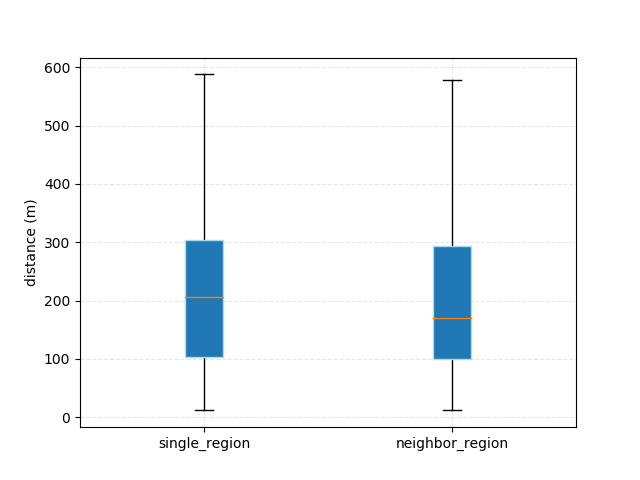
\includegraphics[height=0.3\textheight,width=0.7\textwidth]{figures/平峰车乘匹配}
  \caption{平峰期单独区域调度和邻居区域调度车乘距离对比}\label{fig:pingRegionDistance}
\end{figure}

\begin{figure}[h]
  \centering
  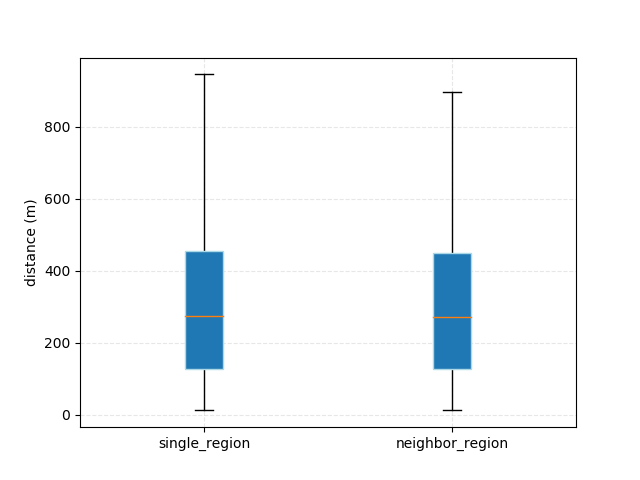
\includegraphics[height=0.3\textheight,width=0.7\textwidth]{figures/低谷车乘匹配}
  \caption{低谷期单独区域调度和邻居区域调度车乘距离对比}\label{fig:shaoRegionDistance}
\end{figure}

高峰期车乘匹配的结果如图\ref{fig:highRegionDistance}所示,单独区域调度比邻居区域调度的车乘距离分布更离散,邻居区域调度的车乘平均距离比单独区域调度缩短了3.07$\%$。在平峰期(如图\ref{fig:pingRegionDistance}所示),邻居区域调度方法中,车辆与乘客距离的中位数比单独区域调度低16.91$\%$。在低谷期(如图\ref{fig:shaoRegionDistance}所示),两种区域调度方式的车乘距离没有太大区别,邻居区域匹配的车乘平均距离只比单独区域匹配低0.43$\%$。

单独的6位区域调度只能调度到自己所属地理区域内的车辆,当乘客所处的位置位于6位GeoHash地理区域的边缘时,如果这个区域内车辆的数目不够,有部分乘客的打车请求不会被满足,但实际上乘客附近的其它6位GeoHash区域中有空车,而且相距乘客的距离也合适,但因为地理划分的问题没有被考虑。6位邻居区域调度可以根据乘客的位置调度到乘客所处区域和周围邻居区域内最近的空车,减少GeoHash划分的地理区域的限制,能够更好地满足乘客的打车需求。

实验数据表明,6位邻居调度调度结果比单独6位GeoHash区域调度结果在分布上更集中,在数值上略有优势。这是因为邻居区域调度优化了单独区域调度的边界限制,乘客在6位GeoHash地理区域边缘可以匹配到邻居区域内实际距离更近的车辆,而不是匹配到本区域内更远的车辆。总而言之,邻居区域调度在车辆调度方面比单独的区域调度更适合应用在出租车调度系统中。

\section{传统区块链与地理位置区块链的系统对比实验}
\subsection{基于模拟道路的系统响应性能对比实验}
系统测试实验从实际应用的方面探究本文所提出方法的正确性和实用性。分为模拟道路的系统实验和真实道路的系统实验两部分。

贾兴无\upcite{贾兴无2018基于网约车数据的居民出行需求特征分析及需求预测}的工作分析了工作日居民选择出租车出行的供需图,其工作统计出,在高峰时段,乘客的出行需求数目可达同时段空驶出租车供给数目的约1.5倍,在平峰时段,乘客的出行需求数目仅仅略高于空驶出租车的供给数目。贾的工作将城市核心区根据不同的土地性质划分为居住区、商业区等交通小区,交通小区的直径在0.5km到2.5km之间,工作日各交通小区的高峰某时刻的出租车需求频数在20至200之间,高峰期各个交通小区每小时的出租车需求频数在60至600之间,本文的系统测试选取2.5km规模的区域进行调度系统的初始化和运行,观察本文所提出的理论工具的实际效果。

系统首先测试了交通小区内高峰期不同初始化车辆状态时,基于传统区块链的全局调度和基于地理位置区块链的区域调度之间的性能差别。考虑到交通小区的范围在0.5km到2.5km之间,选取一个5位GeoHash地图瓦片覆盖的交通小区,交通小区内的道路采用模拟真实路段数据的双行道,小区内每个6位GeoHash瓦片覆盖4个十字路口。在交通小区内模拟高峰期的打车时刻,乘客的出行数量为空驶出租车供给数量的1.5倍,车辆的位置和乘客的上车点在区域内随机均匀分布。保持高峰时刻车辆和乘客的比例,改变两者的数值,得到高峰时传统区块链环境和地理位置区块链环境下系统运行的响应性能对比图\ref{fig:compare}。

\begin{figure}[h]
  \centering
  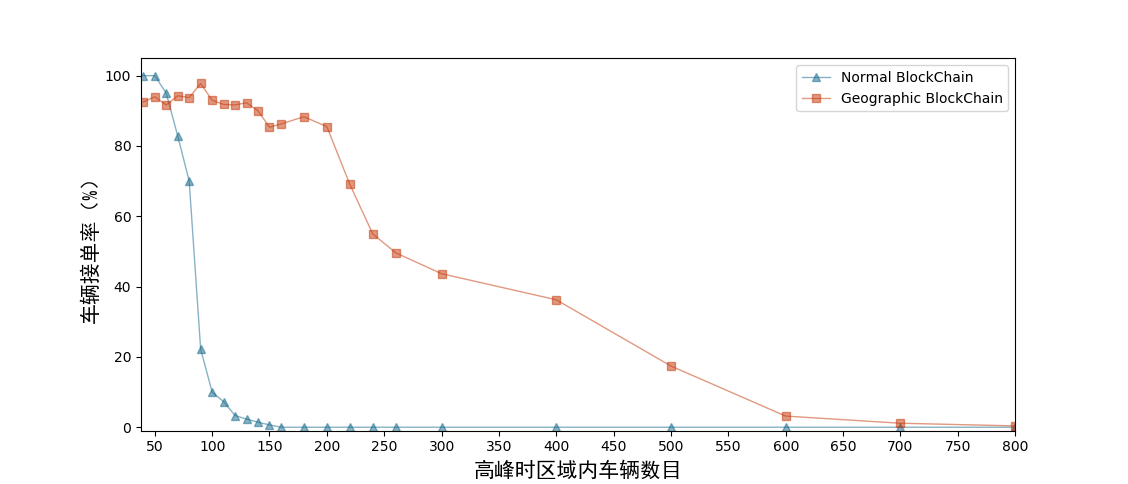
\includegraphics[width=1.0\textwidth]{figures/性能对比}
  \caption{传统区块链与地理位置区块链性能对比}\label{fig:compare}
\end{figure}

横轴为高峰期初始时刻交通小区内初始化的车辆数目(乘客需求数量保持为车辆数量的1.5倍),纵轴为高峰期时,乘客发出请求后,交通小区内接到订单的车辆的比率。在传统区块链中,乘客申请调度车辆时,区块链合约维护的车辆信息过多,遍历车辆信息时会发生超时现象,此时乘客呼叫车辆的请求无法得到响应,导致区域内车辆获取不到乘客的打车信息,接单率不理想。上图在区域内初始化车辆数目为50左右时,传统区块链环境下的车辆接单率为100$\%$,此时区域内所有乘客呼叫车辆不会发生超时。当区域内初始化的车辆数目达到160的规模时,传统区块链后台超过负载极限,无法正常响应交通小区内所有的乘客打车请求,区域内的空驶车辆无法接到订单。

​在地理位置区块链做后台的环境下,由于地理位置区块链后台可以直接查询到乘客附近区域内的车辆账户,避免了对全局的大规模车辆账户进行低效的查询,故响应性能相比传统区块链后台有提升。在区域内车辆分布较多时,地理位置区块链支持的系统中,车辆的接单率平均保持在90$\%$及以上的水平。交通小区内车辆分布数为180辆左右时,所有乘客的打车请求均不会超时。此时若乘客所在附近区域内有空车,乘客呼叫车辆的请求均会得到响应。当交通小区内车辆较少时,在地理位置区块链做后台的环境下,由于部分乘客的邻居区域内没有可调度的空车,故在这一时刻的呼车请求没有得到及时的响应,但该交通小区内所有车辆的接单率仍保持在90$\%$以上的水平。当交通小区内的车辆超过200辆后,乘客的打车请求会有一部分超时,地理位置区块链后台不能及时响应部分请求,导致车辆的接单率下降,此后随着小区内车辆和乘客请求密度的增加,地理位置区块链的响应超时的比例也会增加,直到车辆密度达到800时,区块链后台对所有的请求服务均超时,地理位置区块链后台超过负载极限。

\subsection{基于模拟道路的系统运行数据对比实验}
在传统区块链与地理位置区块链都能支持的出行规模中,在与上述同样规模的交通小区内模拟高峰期持续30min的出行需求,对比两种环境下出租车调度系统运行后的各项指标。初始时区域内有50辆空驶出租车和75个乘客打车需求随机均匀分布,其余的空驶车辆和乘客打车需求在30min内均匀加入到调度系统中,系统运行期间总共处理加入100辆出租车和150位乘客订单,系统运行期间收集的数据信息包括:两种后台环境下的车辆载客时间占比图\ref{fig:timeDistance}(a)、乘客距离接单车辆的距离图\ref{fig:timeDistance}(b)、乘客发出订单到匹配到车辆的响应时间图\ref{fig:manageGas}(a)、区块链后台调度车辆的gas消耗图\ref{fig:manageGas}(b),将收集的数据制作成箱型图进行对比。其中noRegion代表传统区块链后台支持的系统,region代表地理位置区块链后台支持的系统。

\begin{figure}[h]
  \centering
  \subfigure [车辆载客时间占比]{
  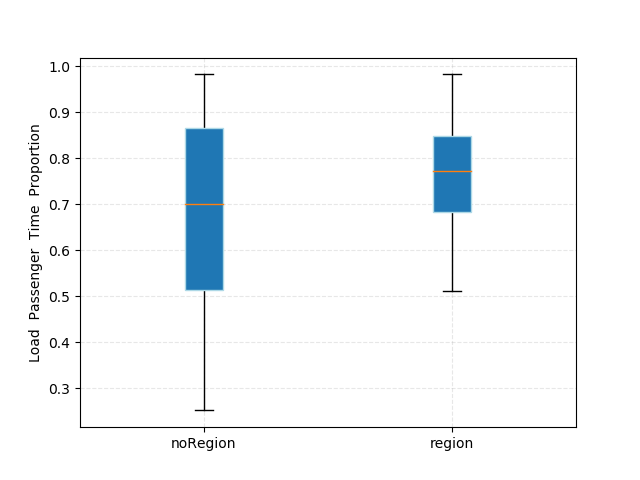
\includegraphics [width=0.45\textwidth]{figures/loadPropotion}}
  \subfigure [乘客和接单车辆的距离]{
  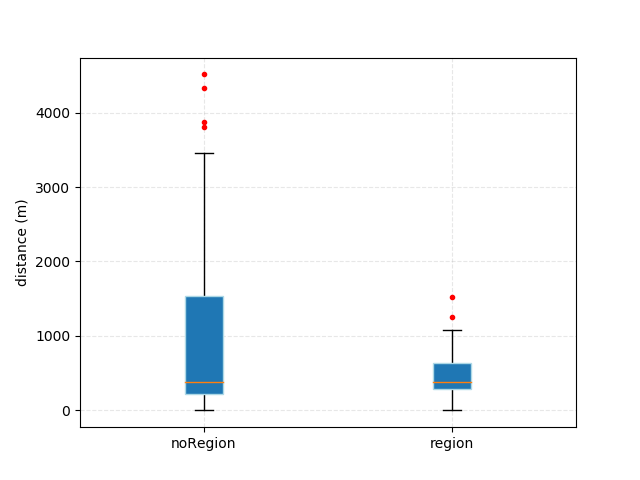
\includegraphics [width=0.45\textwidth]{figures/distance}}
  \caption{载客时间占比和车乘距离对比}
  \label{fig:timeDistance}
\end{figure}

\begin{figure}[h]
  \centering
  \subfigure [乘客匹配到车辆的响应时间]{
  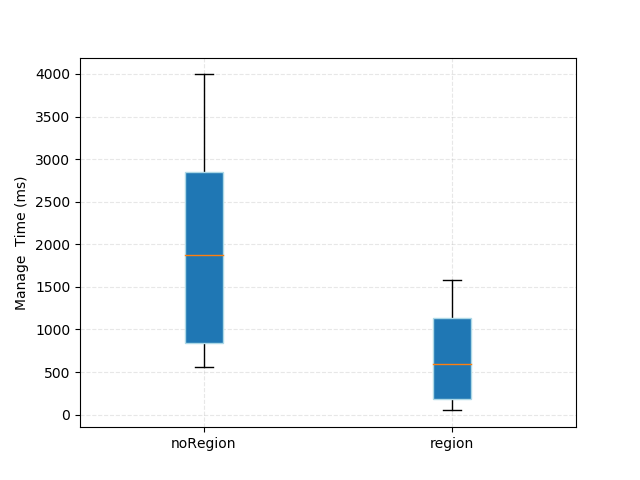
\includegraphics [width=0.45\textwidth]{figures/manageTime}}
  \subfigure [调度车辆的gas消耗]{
  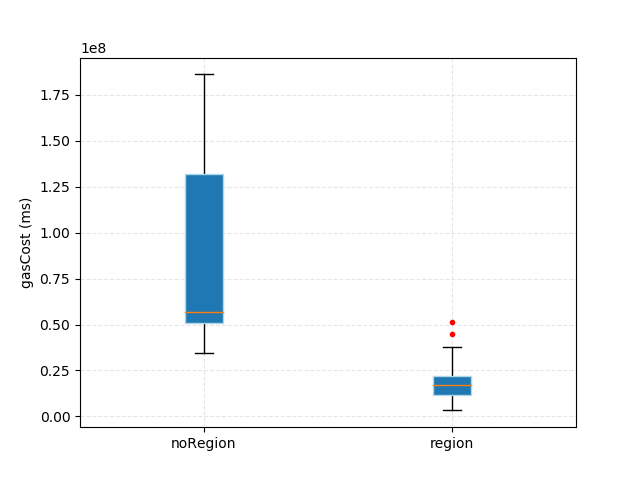
\includegraphics [width=0.45\textwidth]{figures/gasCost}}
  \caption{响应时间和gas消耗对比}
  \label{fig:manageGas}
\end{figure}

车辆载客时间占比箱型图\ref{fig:timeDistance}(a),纵轴为载客时间占车辆订单运行时间的比例,横轴为两种环境下完成订单的同一批车辆个体。从数据统计箱型图可以看到,在地理位置区块链环境下,车辆的载客时间占比更长的情况更多,同时,地理位置区块链区域调度的车辆的载客时间占比分布更集中在0.7及以上,说明在地理位置区块链环境下,大部分出租车的有效载客时间整体得到提高,同一批车辆的载客时间占比中位数,在地理位置区块链环境下比在传统区块链环境下高9.45$\%$,平均值高12.12$\%$,这说明基于地理位置区块链区域调度方法会优化交通小区内车辆的运营效率。

车乘距离箱型图\ref{fig:timeDistance}(b),反映了车辆在接单时与乘客的距离,从图中分析可知,两种环境下,基于地理位置区块链的区域调度的车乘距离的中位数与传统区块链相近,但区域调度的环境下,车辆与乘客的距离数值分布在较小的范围内,90$\%$以上的接单车辆分布在与乘客距离1000米以内,在传统区块链环境中,乘车距离的分布更为离散,有一部分接单的车辆相距乘客的距离达到了3000米以上,这明显降低了一部分乘客的打车体验。相比之下,区域调度可以更有效地在合理的区域范围内调度到距离乘客更近的车辆,平均距离减少了53.73$\%$,让区域内乘客等车的时间减少,优化了乘客的打车感受。

乘客打车响应时间箱型图\ref{fig:manageGas}(a),反映了乘客发出订单后,到接受服务端返回的匹配到的车辆信息的时间间隔。由图可知,全局调度环境下的打车响应时间相较于区域调度环境下更加离散,区域调度在打车响应时间的指标上具有明显的优势,区域调度车辆的响应时间中位数在600ms左右,全局调度车辆的响应时间中位数在1800ms左右。同时,全局调度中还有部分乘客的响应时间接近4000ms,这是由于全局调度考虑的车辆数目较多,后台修改记录状态的开销增加,导致响应时间增加。在后台运算的gas消耗上,区域调度进行车乘匹配的运算消耗平均是全局调度gas消耗的20.93$\%$。

\subsection{基于真实道路的系统运行数据对比实验}
保持交通小区的规模不变,选取北京市海淀区以大钟寺地铁站为中心,东西长4km、南北长5km的一块地理区域,基于该区域的道路和路口在真实地图数据中运行出租车调度系统。模拟高峰期持续30min的出行需求,初始时区域内有50辆空驶出租车和75个乘客打车需求在路口随机均匀分布,其余的空驶车辆和乘客打车需求在30min内均匀加入到调度系统中,系统运行期间总共处理加入100辆出租车和150位乘客订单,系统运行期间收集的数据信息如下:两种后台环境下的车辆载客时间占比图\ref{fig:real_timeDistance}(a)、乘客距离接单车辆的距离图\ref{fig:real_timeDistance}(b)、乘客发出订单到匹配到车辆的响应时间图\ref{fig:real_manageGas}(a)、区块链后台调度车辆的gas消耗图\ref{fig:real_manageGas}(b)。

\begin{figure}[h]
  \centering
  \subfigure [车辆载客时间占比]{
  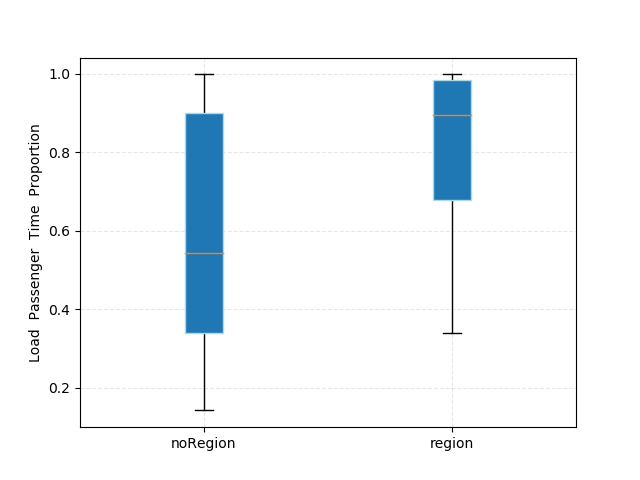
\includegraphics [width=0.45\textwidth]{figures/real_routeTime}}
  \subfigure [乘客和接单车辆的距离]{
  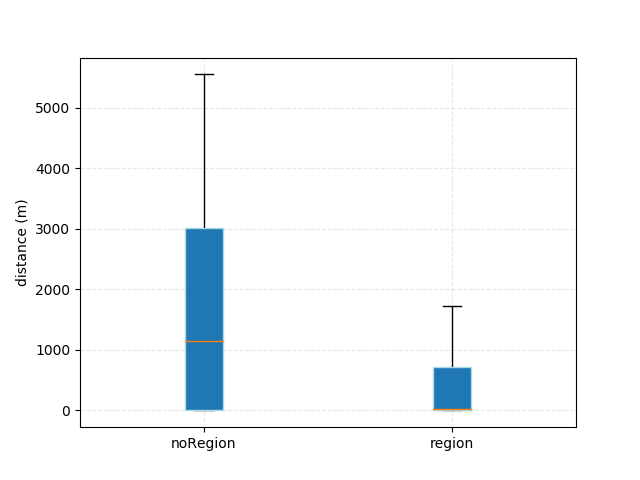
\includegraphics [width=0.45\textwidth]{figures/real_distance}}
  \caption{真实道路中载客时间占比和车乘距离对比}
  \label{fig:real_timeDistance}
\end{figure}

\begin{figure}[h]
  \centering
  \subfigure [乘客匹配到车辆的响应时间]{
  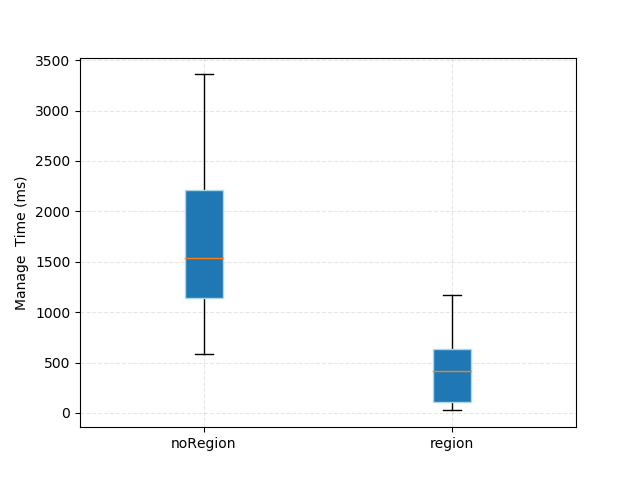
\includegraphics [width=0.45\textwidth]{figures/real_manageTime}}
  \subfigure [调度车辆的gas消耗]{
  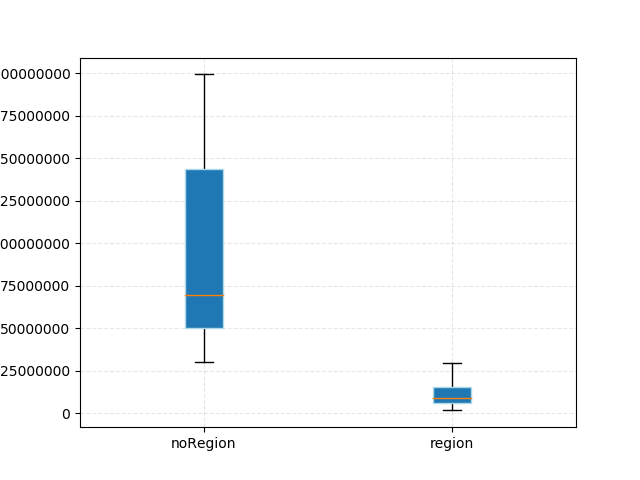
\includegraphics [width=0.45\textwidth]{figures/real_gasCost}}
  \caption{真实道路中响应时间和gas消耗对比}
  \label{fig:real_manageGas}
\end{figure}

收集真实道路下系统运行的数据分析可知,基于地理位置区块链的系统较传统区块链的系统,车辆的平均载客时间高37.2$\%$,乘客打车的响应时间平均减少了74.9$\%$,匹配到的车辆相距乘客的距离结果分布更集中,且平均距离减少了77.4$\%$。这是因为在真实道路中做实验时,车辆和乘客上车点的位置均选在道路的路口,而路口处的各个位置点之间距离较近,故乘客通过邻居区域调度匹配到距离较近的车辆后,距离优化和车辆载客时间占比优化的效果会更明显。基于真实地图数据的实验更能说明应用地理位置区块链进行区域调度的优越性,其特性在真实地图的场景中得到了验证。

\section{系统测试实验}
\subsection{地理位置区块链性能测试实验}
本部分旨在探究一个地理位置区块链服务节点并发处理乘客打车请求的能力。实验设置了8 × 10km的区域,在区域内维护足够多的车辆,初始化1000辆空车在区域内均匀分布,目的是保证每个乘客在进行6位邻居区域调度时都能够匹配到车辆。改变区域内同时发出请求的乘客数量,每增加10个乘车请求为一组,乘客请求的上车点在区域内均匀分布。在处理完毕同时并发的乘车请求后,统计未完成的订单的数目,以此来探究区块链节点能够并发处理的乘客请求规模。
% 区域规模、请求规模,探究不同区域下可以请求多大的规模。探究更大范围的地理区域可以支持多大规模的车乘交互请求,

\begin{figure}[h]
  \centering
  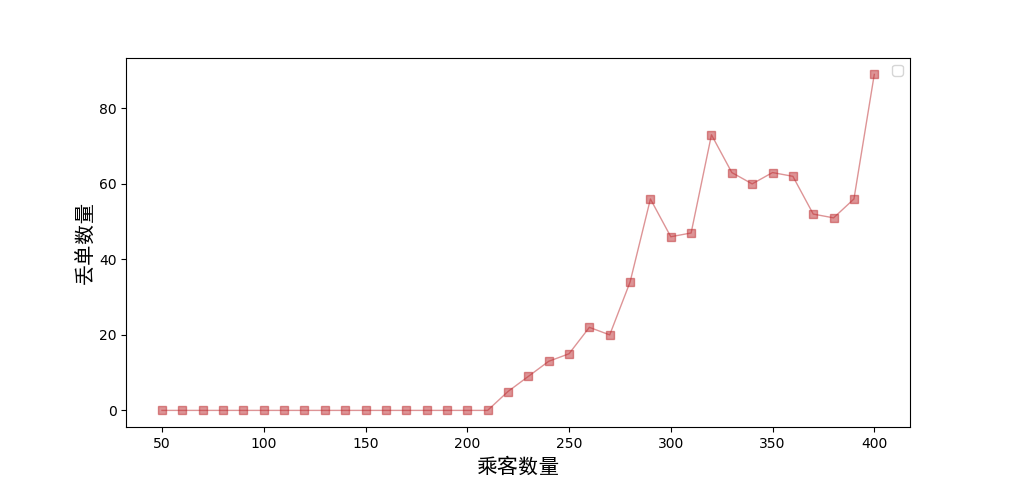
\includegraphics[width=1.0\textwidth]{figures/地理位置区块链性能实验}
  \caption{地理位置区块链性能实验}\label{fig:treeBlockchcainPerformance}
\end{figure}

如图\ref{fig:treeBlockchcainPerformance},在同时向同一服务节点发出请求的乘客规模在210个以下时,所有的乘客订单均被完整执行,没有出现请求车辆超时或者导航超时的现象。当同时发出请求的乘客规模达到220个时,有5个乘客订单未被完成。其原因是乘客匹配到的车辆在向服务节点请求导航路径的过程中,返回路径规划结果超时,导致车辆没有完成完整的订单。此后随着乘客请求规模的增大,未完成订单的数量也随之逐渐增加。由于乘客上车点分布的随机性,乘客的请求规模扩大后,未完成的订单随之增加的趋势并不是线性的,但仍能反映出后台节点处理乘客请求能力逐渐下降。在未完成的订单中,有一部分是乘客的乘车请求发出后,后台匹配车辆超时,其余订单未完成是因为后台处理车辆的导航请求超时。

实验结果表明,一个地理位置区块链服务节点,在同时服务规模为200的乘客打车请求时,其处理车辆调度的业务请求均不会发生超时。故在本实验环境下,一个地理位置区块链服务节点可以服务约200名乘客的并发乘车请求,在此规模下不会发生超时响应。

\subsection{系统在模拟道路上的运行实验}
在4km × 5km的区域范围内,初始化140辆车和200个乘客打车请求,模拟2小时的高峰期出行环境。2小时内该区域共运行560辆车和800个乘客订单,收集运行过程中,乘客和匹配到的车辆的距离、乘客打车的响应时间数据,作为观察系统特征的参考。

\begin{figure}[h]
  \centering
  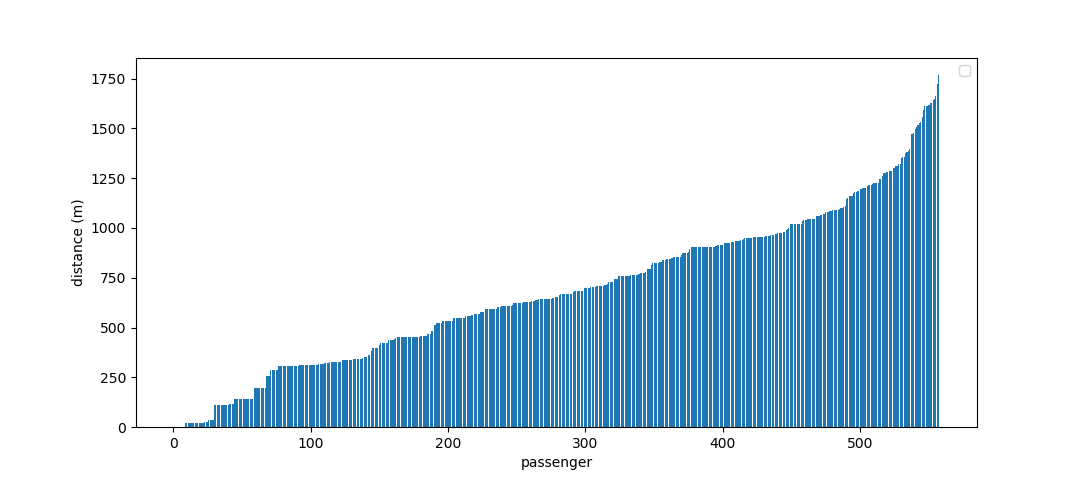
\includegraphics[width=1.0\textwidth]{figures/2hDistance}
  \caption{模拟地图-系统运行2小时车乘距离}\label{fig:2hDistance}
\end{figure}

\begin{figure}[h]
  \centering
  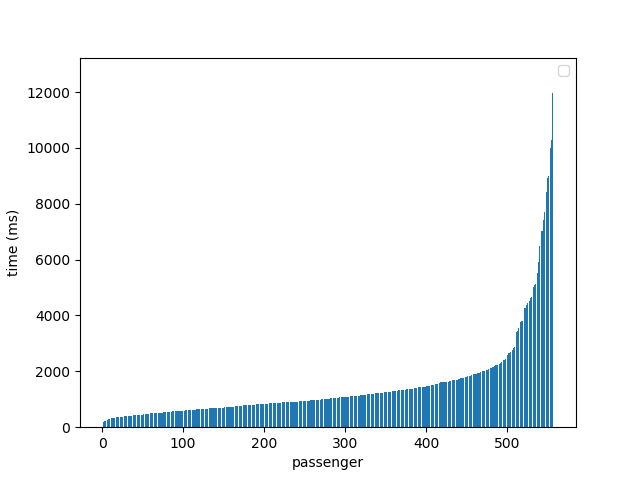
\includegraphics[width=1.0\textwidth]{figures/2hTime}
  \caption{模拟地图-系统运行2小时响应时间}\label{fig:2hTime}
\end{figure}

运行结果数据统计如图\ref{fig:2hDistance}和图\ref{fig:2hTime}。2小时内,呼叫到出租车的乘客,其距离车辆的距离最大为1750m左右,80$\%$以上的车辆与乘客的距离在200m至1200m的范围内,乘客调度出租车的合理距离范围。出租车调度系统系统2小时的运行过程中,乘客呼叫出租车的响应时间,绝大部分在4s以内,最大响应时间不超过12s。

\subsection{系统在真实道路上的运行实验}
选取北京市海淀区以大钟寺地铁站为中心,东西长4km、南北长5km的一块地理区域,基于该区域的道路和路口在真实地图数据中运行出租车调度系统,与模拟道路实验的条件相同,初始化140辆车和200个乘客打车请求,模拟2小时的高峰期出行环境。2小时内该区域共运行560辆车和800个乘客订单,收集系统运行过程中,乘客和车辆的距离、乘客打车的响应时间数据,作为观察系统特征的参考。

\begin{figure}[h]
  \centering
  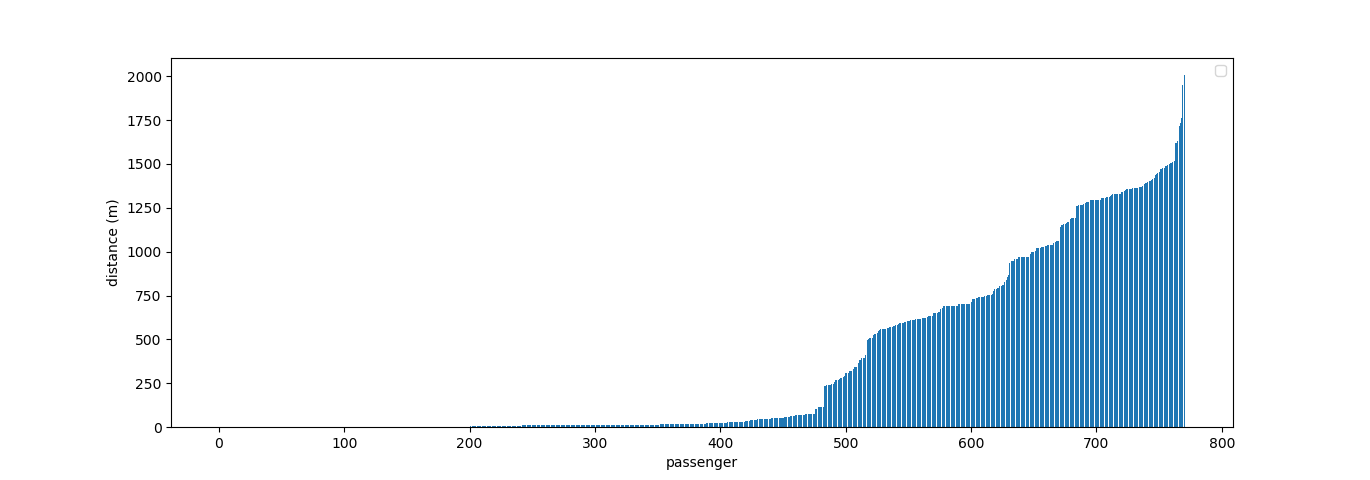
\includegraphics[width=1.0\textwidth]{figures/real_2hDistance}
  \caption{真实地图-系统运行2小时车乘距离}\label{fig:real_2hDistance}
\end{figure}

\begin{figure}[h]
  \centering
  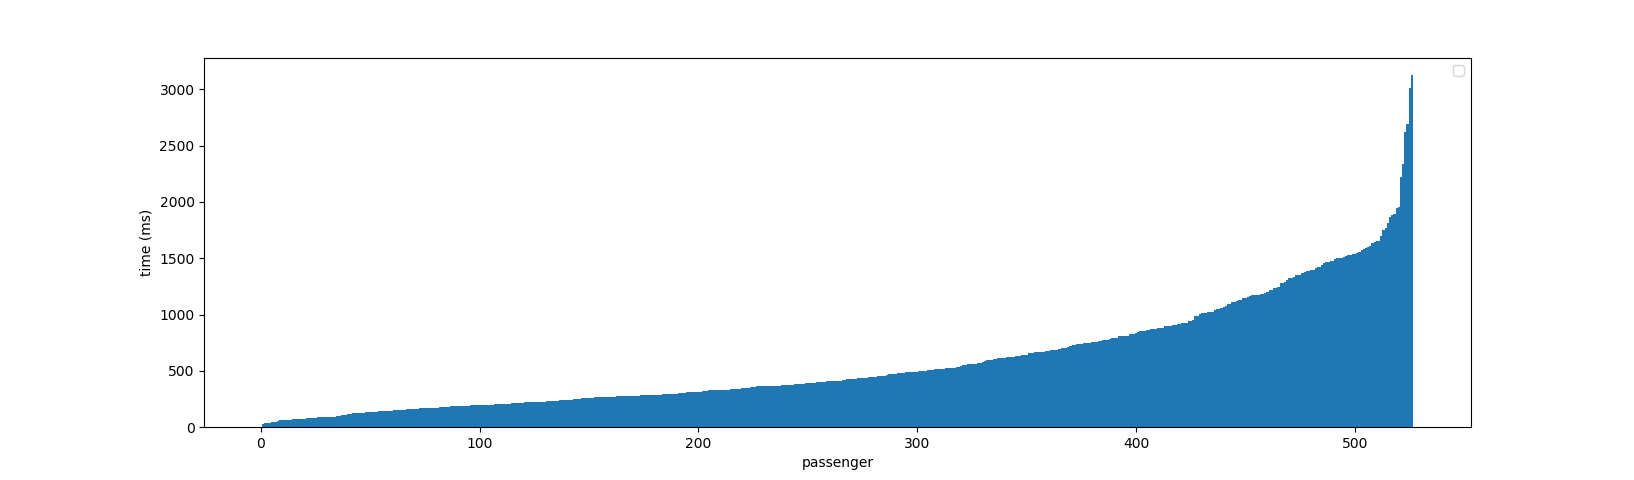
\includegraphics[width=1.0\textwidth]{figures/real_2hTime}
  \caption{真实地图-系统运行2小时响应时间}\label{fig:real_2hTime}
\end{figure}

运行结果数据统计如图\ref{fig:real_2hDistance}和图\ref{fig:real_2hTime}。分析交通系统的运行结果可知,系统在2小时的运行过程中,乘客距离其匹配到的车辆最远距离在2000m左右,80$\%$以上的车辆与乘客的距离在1500m的范围内。乘客呼叫出租车的响应时间不超过5s。出租车调度系统在真实地图环境的运行中的结果,包括乘客打车响应时间、车辆相距乘客的距离、车辆的载客时间占比等均处在合理的范围内。说明本出租车调度系统可以在真实的地图数据中正常运行并得到合理的结果。本工作将地理信息与区块链相结合,简化了计算方式,优化了计算效率,并且可以基于地理信息设计有效的方法来研发应用,有效验证了结合地理信息的区块链在车载自组网方向上的实用性。

\section{本章小结}
本章首先对系统的算法特征进行了实验验证,通过实验证明了距离计算优化算法对GeoHash几何计算效率的提升。接着,本章5.2节对后台智能合约的路径规划算法进行了实验测试和参数调节,以选出适合出租车调度系统的算法精度来提高算法效率。之后,在5.3节,本章对基于地理位置区块链的单独区域调度算法和邻居区域调度算法进行了对比实验,证明了邻居区域调度算法更适合出租车调度系统。本章的5.4节,对比了传统区块链和地理位置区块链环境下进行出租车调度的系统性能,然后在两种环境都支持的业务规模下进行了模拟道路和真实道路的系统运行实验,并将两种环境下的实验结果进行对比,证明了采用地理位置区块链进行区域调度的系统更具健壮性和高效性。本章的5.5节首先通过实验测试了地理位置区块链后台能响应的并发请求的规模,然后在地理位置区块链后台能够正常响应的规模下进行了模拟道路和真实道路的系统测试。系统测试的结果表明,出租车调度系统的车辆调度结果和响应时间均处在合理范围内,证明了系统的实用性,同时也验证了基于地理位置区块链设计车载自组网应用的可行性。


%%==================================================
%% conclusion.tex for BIT Master Thesis
%%==================================================


\begin{conclusion}

智能汽车的广泛使用,使得车辆之间的联系越来越紧密,车辆之间要传递大量信息的需求,使得车载自组网的应用成为可能。利用车载自组网,将智能车辆组织起来,分享和传递数据。车载自组网需要建立去中心化的 ad-hoc 网络,而区块链具备去中心化、不可篡改、共识机制等特点,所以将区块链技术用于车载自组网中是一种可行方案。然而,车载自组网需要与地理信息密切结合,且自组网中的节点具备移动性的特点。传统区块链的存储结构并不能够很好的解决上述问题。另外,车载自组网的大量应用都与地理位置信息和身份信息密切相关,而数据来源于开放的互联网平台,存在被篡改的风险,且传统的地理信息以经纬度的形式在矢量地图表示,在区域信息绑定、信息安全等问题上存在问题。现有的基于区块链的车辆调度研究工作,大多是针对基于区块链的身份验证机制和零知识信任机制进行研究,或是针对区块链节点在性能方面的处理能力进行研究,缺乏对实际的地图数据、调度机制和业务场景进行实际应用的探索。

针对上述问题,本文完成了对区块链相关工作的调研,并对地理位置区块链的研究进行了介绍。同时,本文对地图信息的存储、展现和使用进行了相关研究,拓展了GeoHash矢量地图的相关功能,在区块链平台实现了继续GeoHash矢量地图的路径规划算法,基于地理位置区块链平台设计了出租车调度的匹配机制,并在此基础上实现了完整的出租车调度系统设计,将该系统与传统区块链环境下的调度系统作对比。此外本文还对基于地理位置区块链的调度系统性能做了实验探究,以及在模拟环境和真实道路的环境下对系统的实用性进行了测试和验证。本文的主要工作总结如下:

1. 增加了GeoHashTile地图的功能,实现了leaflet地图工具从屏幕坐标点到地理位置GeoHash点的投影过程,并在此基础上实现了对GeoHash矢量地图的放缩和拖动功能,优化了GeoHash矢量地图的展示效果,更有利于GeoHash矢量地图的研究和实际应用。

2. 优化了基于GeoHash的距离计算方法,优化了合约端的计算速度,降低了计算的gas开销,从而降低了区块链平台的计算压力,更有利于在区块链平台上进一步实现出租车调度系统。

3. 设计并实现了基于GeoHash矢量地图的路径规划算法,并根据GeoHash位置数据的特点对算法的计算参数进行优化,在保证路径规划结果正确性的同时,提高了算法的计算效率,降低了区块链平台的运算量,更有利于系统实现。

4. 设计并实现了基于地理位置区块链的区域调度方法,实验结果表明地理位置区块链环境下的区域调度方法比传统区块链环境下的全局调度方法具有更强的拓展性。地理位置区块链服务端支持的调度系统车乘交互规模是传统区块链的3倍。在其他条件相同的情况下,地理位置区块链环境支持的系统运行结果,其车辆的有效运行时间、乘客打车的运行时间、匹配到的车辆相距乘客的距离均有优化。本文对调度系统进行规模化测试的运行结果也均处于合理范围,证明了将GeoHash编码、地理信息和区块链相结合的思想,能够良好的适用于车载自组网的实际应用。

本文的工作仍有可拓展的研究方向和补足之处:
可以探究区块链的准入机制和零知识证明机制,在用户安全的层面加强系统的安全性。另外,为了加强出租车调度系统与实际地理信息的结合,可以将实时路况的维护与路径规划算法相结合,通过区块链本身的特点增强路况结果的安全性和可信性,同时让导航结果更具备参考性和实用性。此外,可以在系统中加入对出租车空驶巡航的路线推荐功能,在解决各个时期的乘车资源分配问题方面做出探究,更有效地利用地理信息与区块链相结合的特点,提升交通系统的运行效率。

\end{conclusion}

%% 参考文献,五号字,使用 BibTeX,包含参考文献文件.bib

%\bibliography{reference/chap1,reference/chap2} %多个章节的参考文献
\bibliography{reference/chap1,reference/chap2}

%%%%%%%%%%%%%%%%%%%%%%%%%%%%%%
%% 后置部分
%%%%%%%%%%%%%%%%%%%%%%%%%%%%%%

%% 附录(章节编号重新计算,使用字母进行编号)
\appendix
\renewcommand\theequation{\Alph{chapter}--\arabic{equation}}  % 附录中编号形式是"A-1"的样子
\renewcommand\thefigure{\Alph{chapter}--\arabic{figure}}
\renewcommand\thetable{\Alph{chapter}--\arabic{table}}

\include{chapters/app1} 
\include{chapters/app2} 

%(其后部分无编号)
\backmatter

% 发表文章目录
%%==================================================
%% pub.tex for BIT Master Thesis
%% modified by yang yating
%% version: 0.1
%% last update: Dec 25th, 2016
%%==================================================

\begin{publications}{99}
\end{publications}

% 致谢
%%==================================================
%% thanks.tex for BIT Master Thesis
%% modified by yang yating
%% version: 0.1
%% last update: Dec 25th, 2016
%%==================================================

\begin{thanks}

首先,衷心感谢我的导师陆慧梅老师和向勇老师。两位老师在我因迷茫而失落的时候,像灯塔一样为我指明了方向。在我遇到困难而不知所措的时候,教会了我调节心态和解决问题的有效方法。导师对我论文的研究方向提供了宝贵的意见和细心的指导,教会了我如何自我发现和解决问题,教会了我严谨的批判性思维,培养了我在科研工作中的逻辑思维能力和梳理总结能力。导师耐心的指导和教诲是我读研期间最珍贵的收获。

感谢同门的周畅师姐和万琦玲师妹。她们在我论文撰写过程中给予了很多帮助,提出了许多有益的改善性意见。我在科研方向选择和实验的具体细节上,都获得了周畅师姐的诸多帮助。我还要感谢1036实验室的所有老师同学。感谢王馨茹师姐在我一次次情绪失落时对我的安慰和鼓励。感谢雷鑫晨同学带我去健身房强身健体,拓展经历。感谢于长鑫同学教会我容器技术的使用,提高了我做实验搭环境的效率。感谢李祥潮同学和刘金田同学分享的求职经验,让我感受到了大佬们的眼界和本领。感谢曾秋阳同学和孟玲同学的解忧陪聊和关心。实验室的大家在学习过程中互相学习,互相帮忙,共同度过了一段美好难忘的时光。此外,我要感谢辅导员王柳婷对我的帮助,不论是学习课程还是完成毕设期间,她都为学生事务尽职尽责,为我们每一位学生排解烦恼和解决问题。

感谢我的朋友刘浩磊、丁波文和任浩,我们共同拥有一起考研、一起探讨人生目标、一起相互鼓励这些深刻的人生经历。我还要感谢我的舍友许泽松同学,在课程作业中他是得力的伙伴,在一起求职时他是消息灵通的战友。感谢邱柯铭同学,在我遇到困难的时候给了我很多支持和帮助。同时,我也要感谢我的工作参考文献中的作者们。他们的深入研究鞭辟入里,让我在研究课题中找到了很好的出发点。

最后,谢谢论文评阅老师们的辛苦工作,感谢陆慧梅老师、杨松老师、段春晖老师对我学习上的关心和帮助。衷心感谢一直以来陪伴着我的家人、朋友和同学们。正是他们在背后坚定的支持和帮助,我才得以顺利完成此论文。两年时光如白驹过隙,前路漫漫,吾将上下而求索。

\end{thanks}

% 作者简介(博士论文需要)
%%==================================================
%% resume.tex for BIT Master Thesis
%% modified by yang yating
%% version: 0.1
%% last update: Dec 25th, 2016
%%==================================================

\begin{resume}

\end{resume}



\end{document}
